\section[Model Performance]{Spectral ViT Model Performance}
\begin{frame}{Spectral ViT V1}
    \begin{figure}
        \centering
        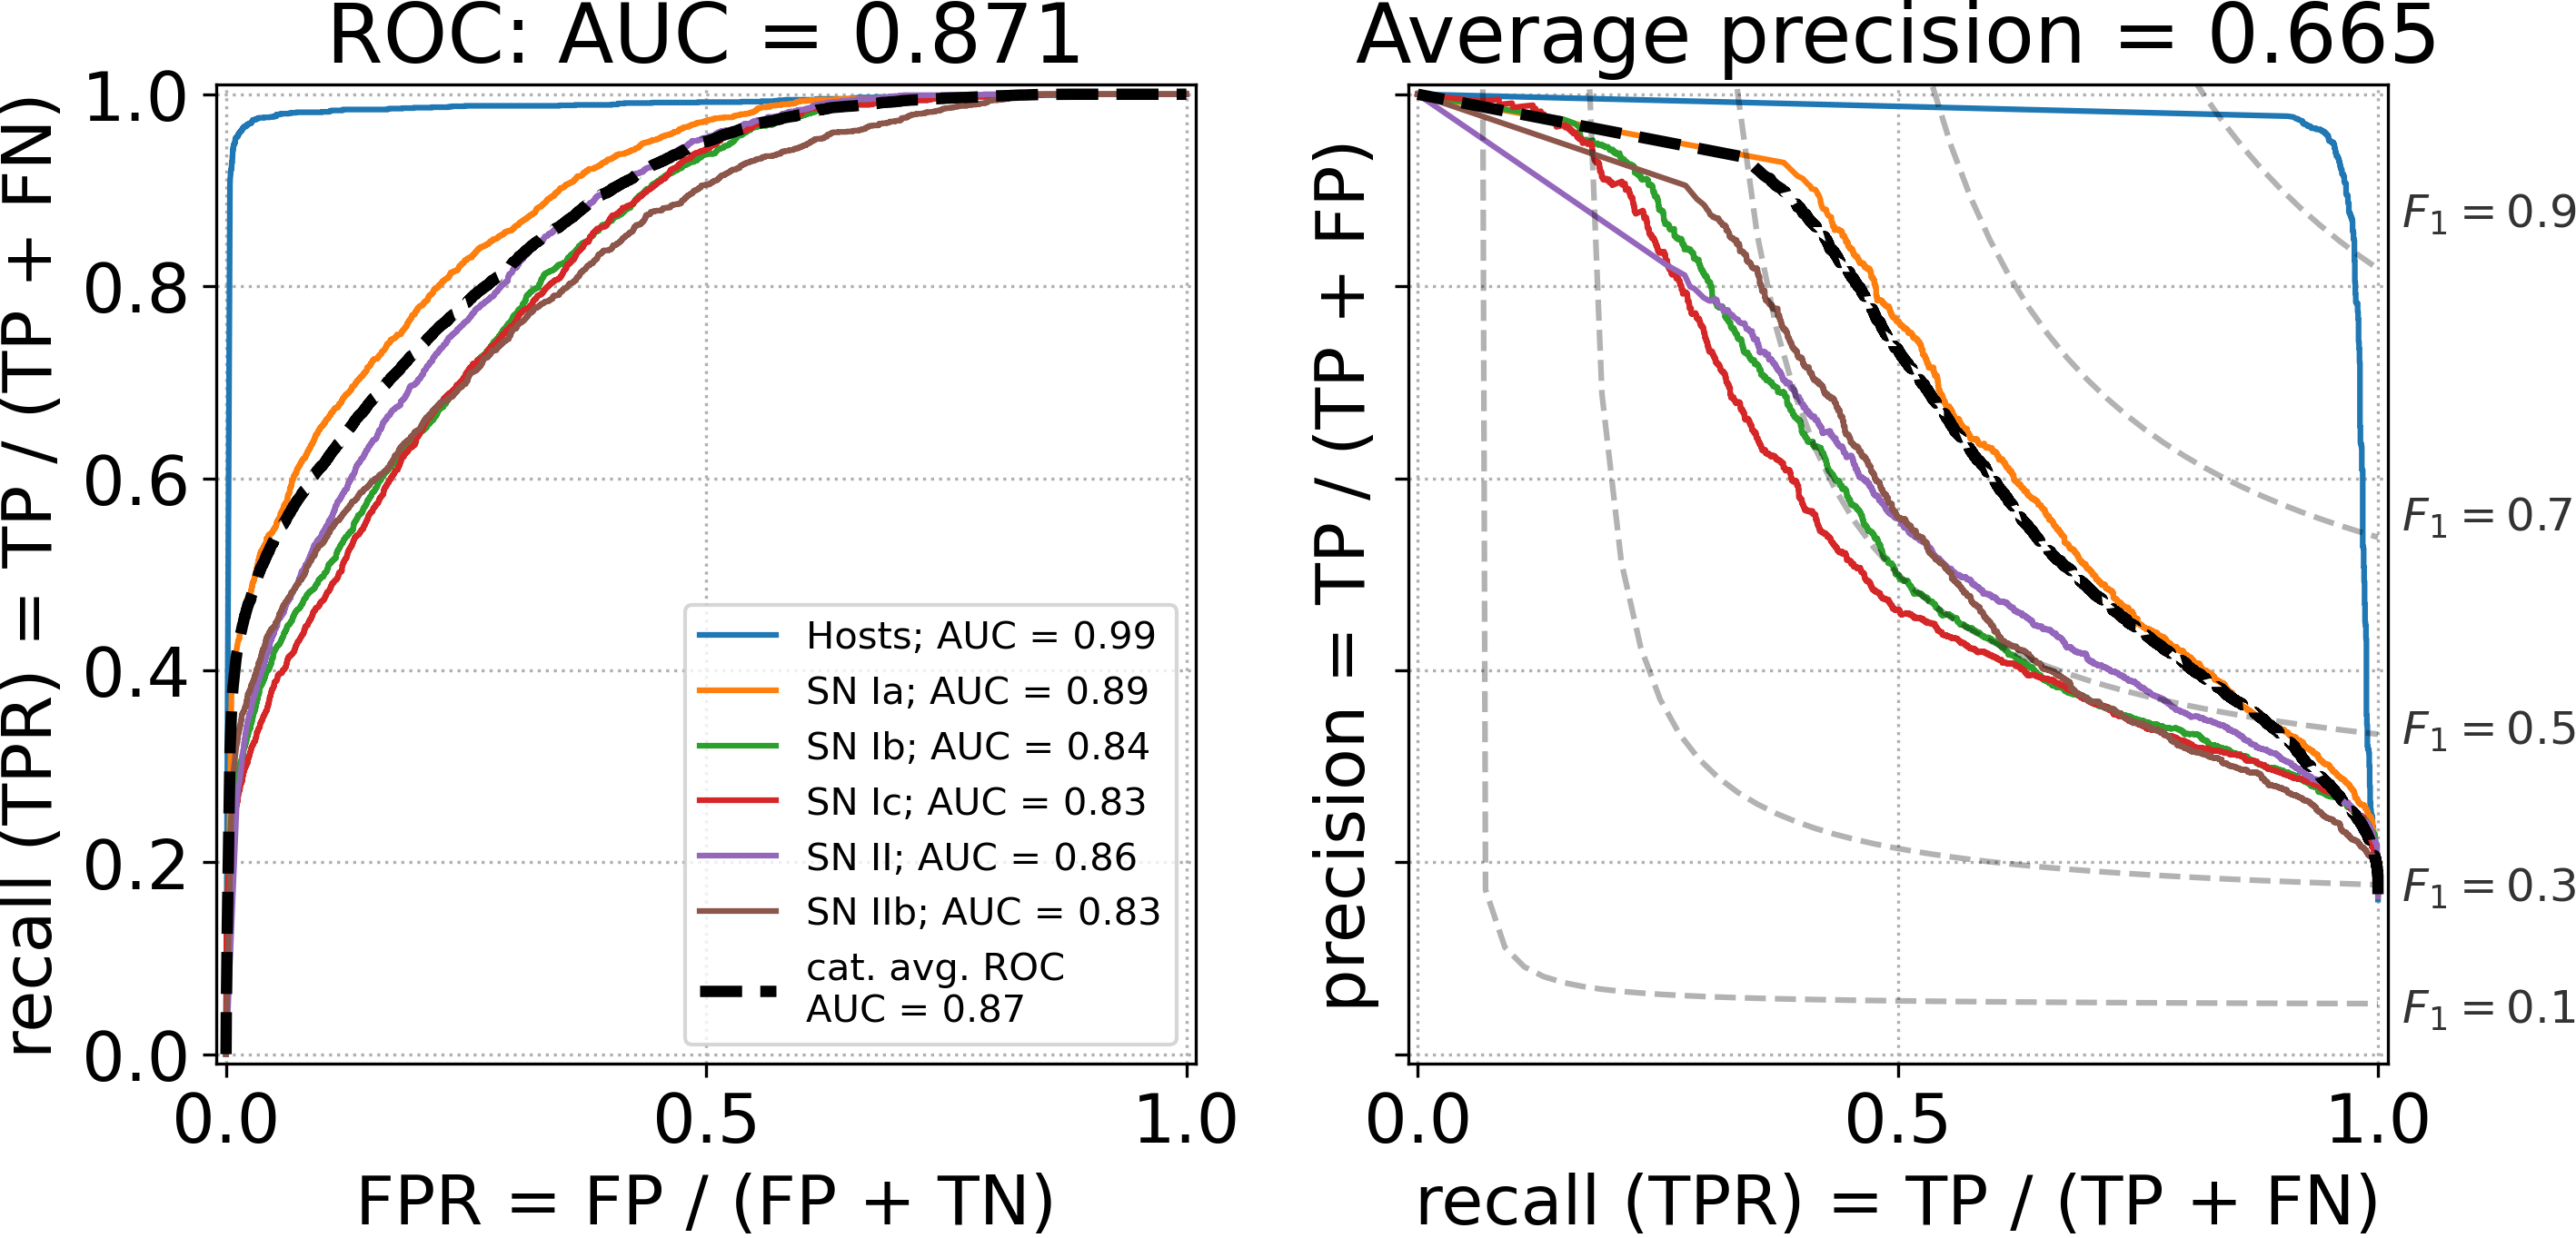
\includegraphics[height=2.8cm]{figures/v1_real/vit_model_V1_original_redorocfulle_e31.png}
        \quad
        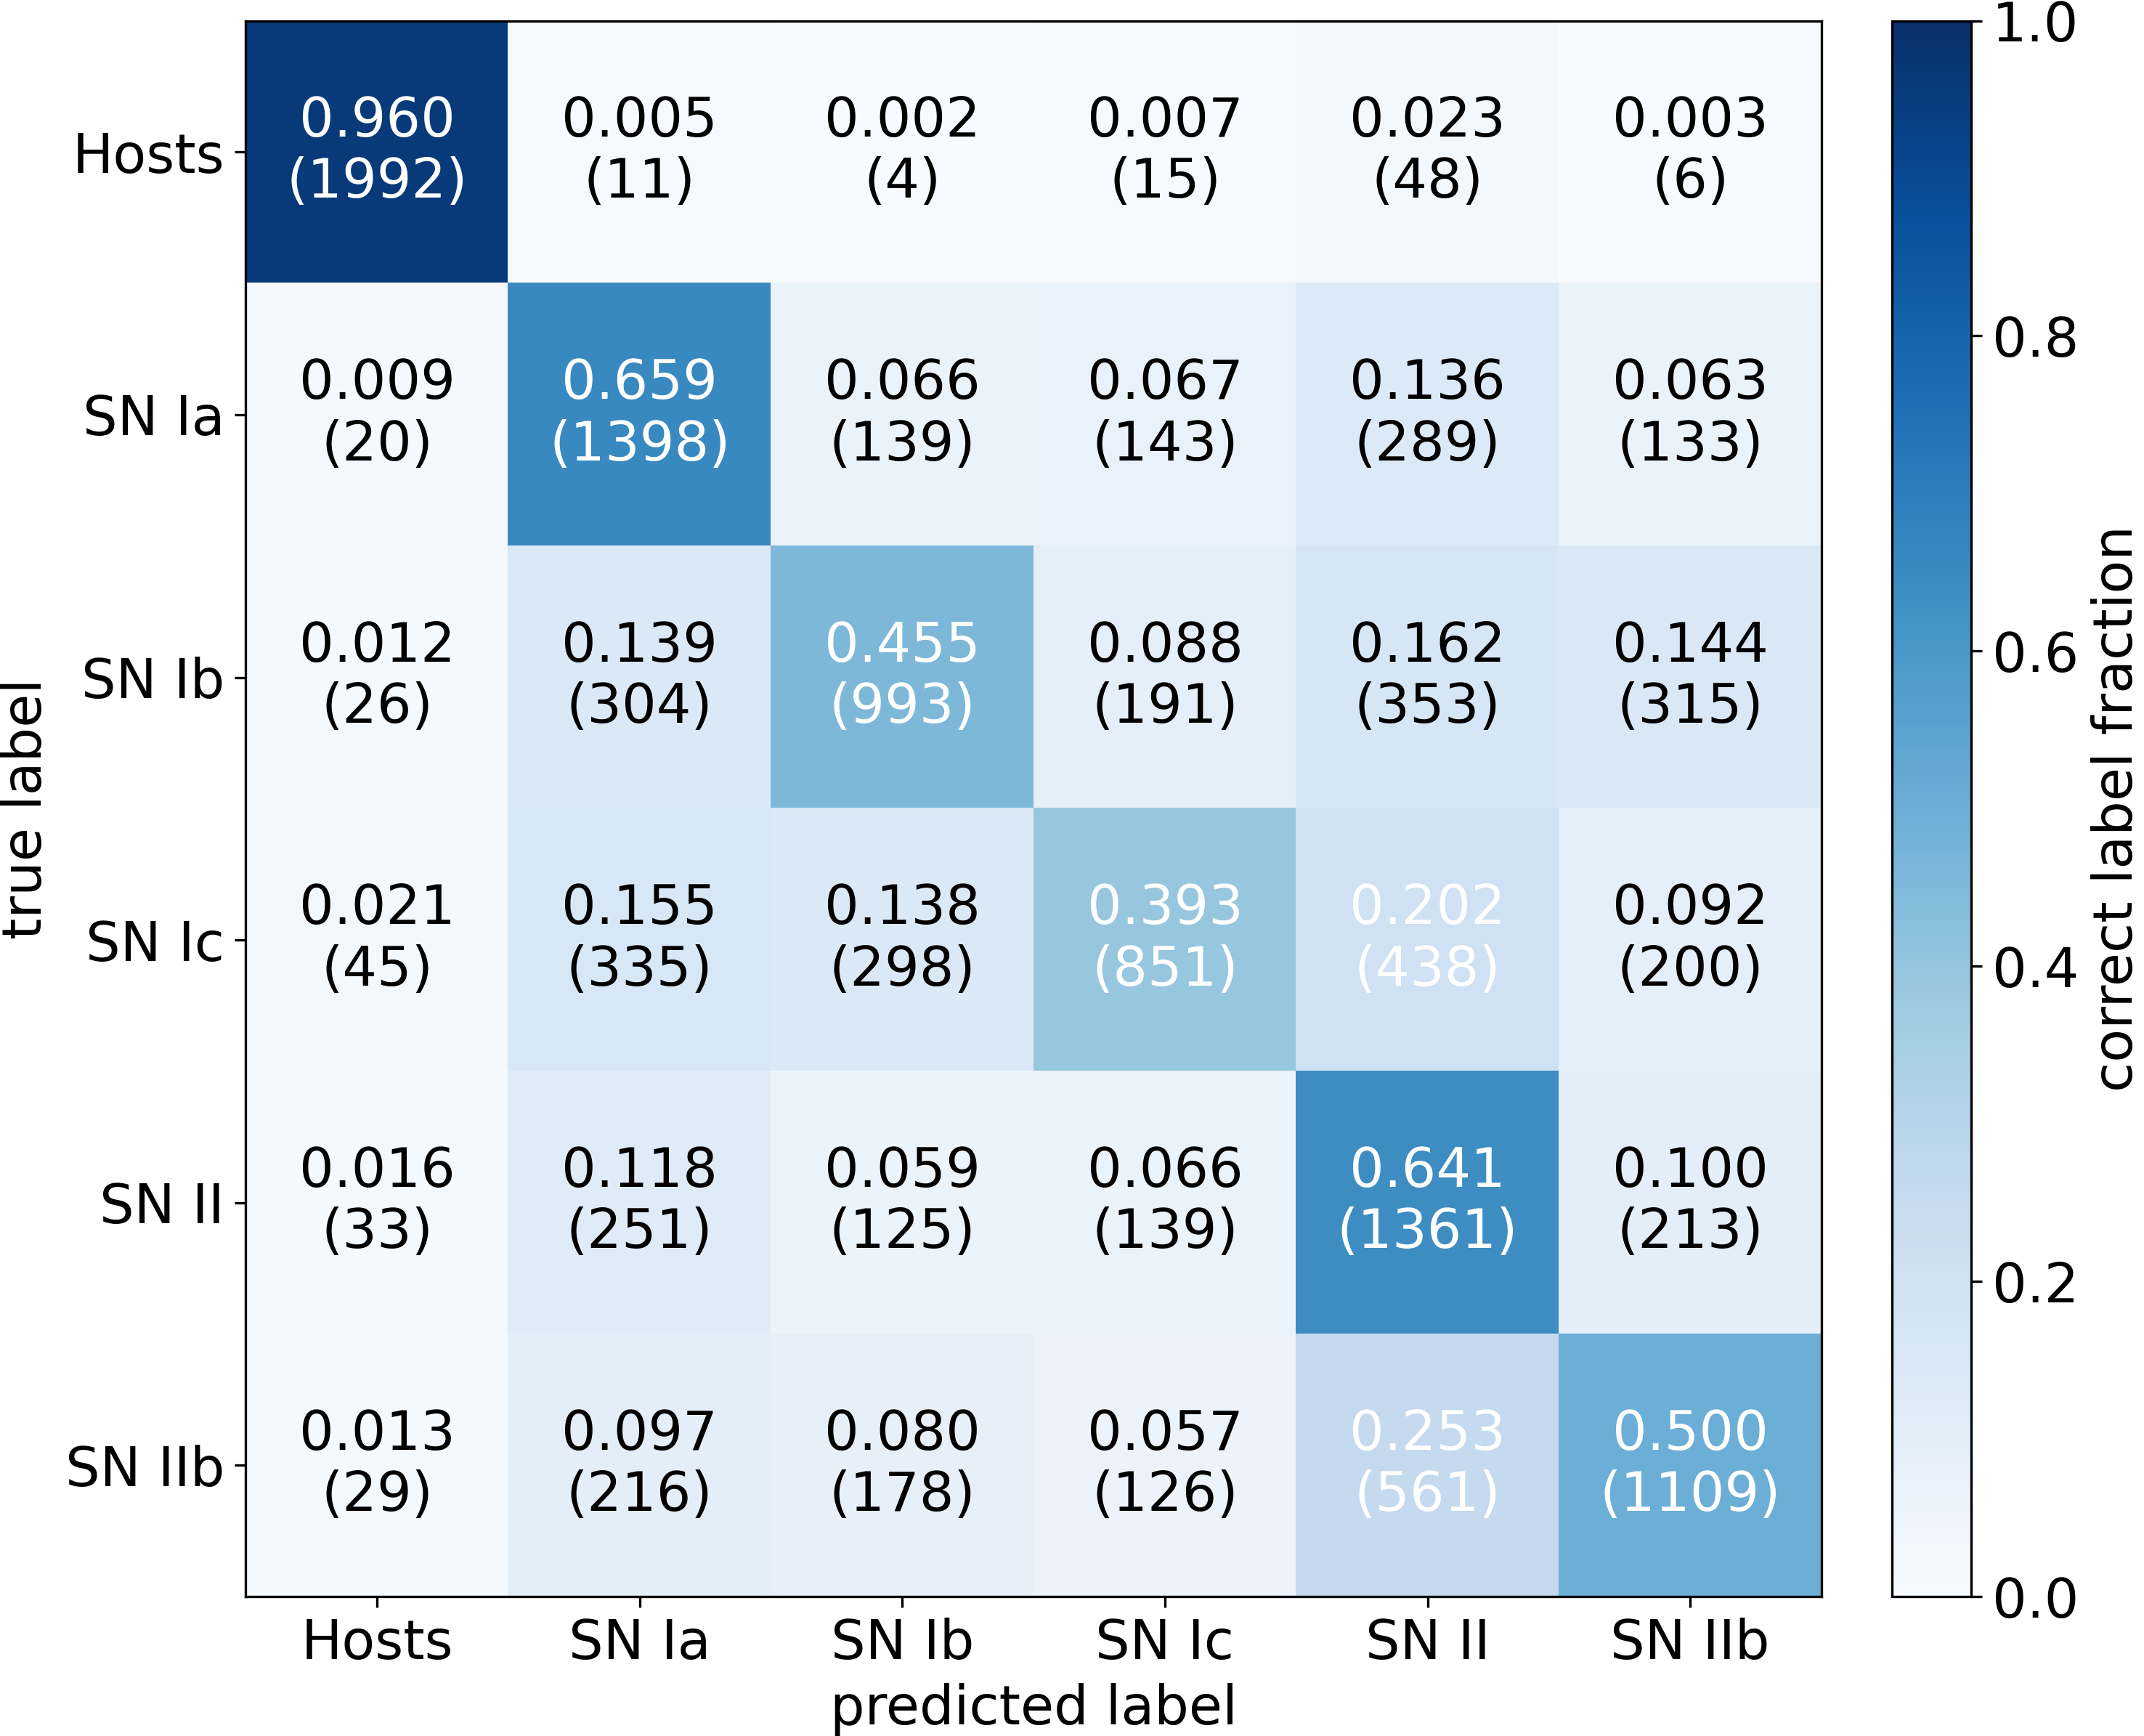
\includegraphics[height=2.8cm]{figures/v1_real/vit_model_V1_original_redocmfull_e31.png}
        \caption{Spectral ViT V1 Classifier\label{fig:v1_qual}}
        \pause
%     \end{figure}
% \end{frame}

% \begin{frame}
%     \begin{figure}[t]
%         \centering
        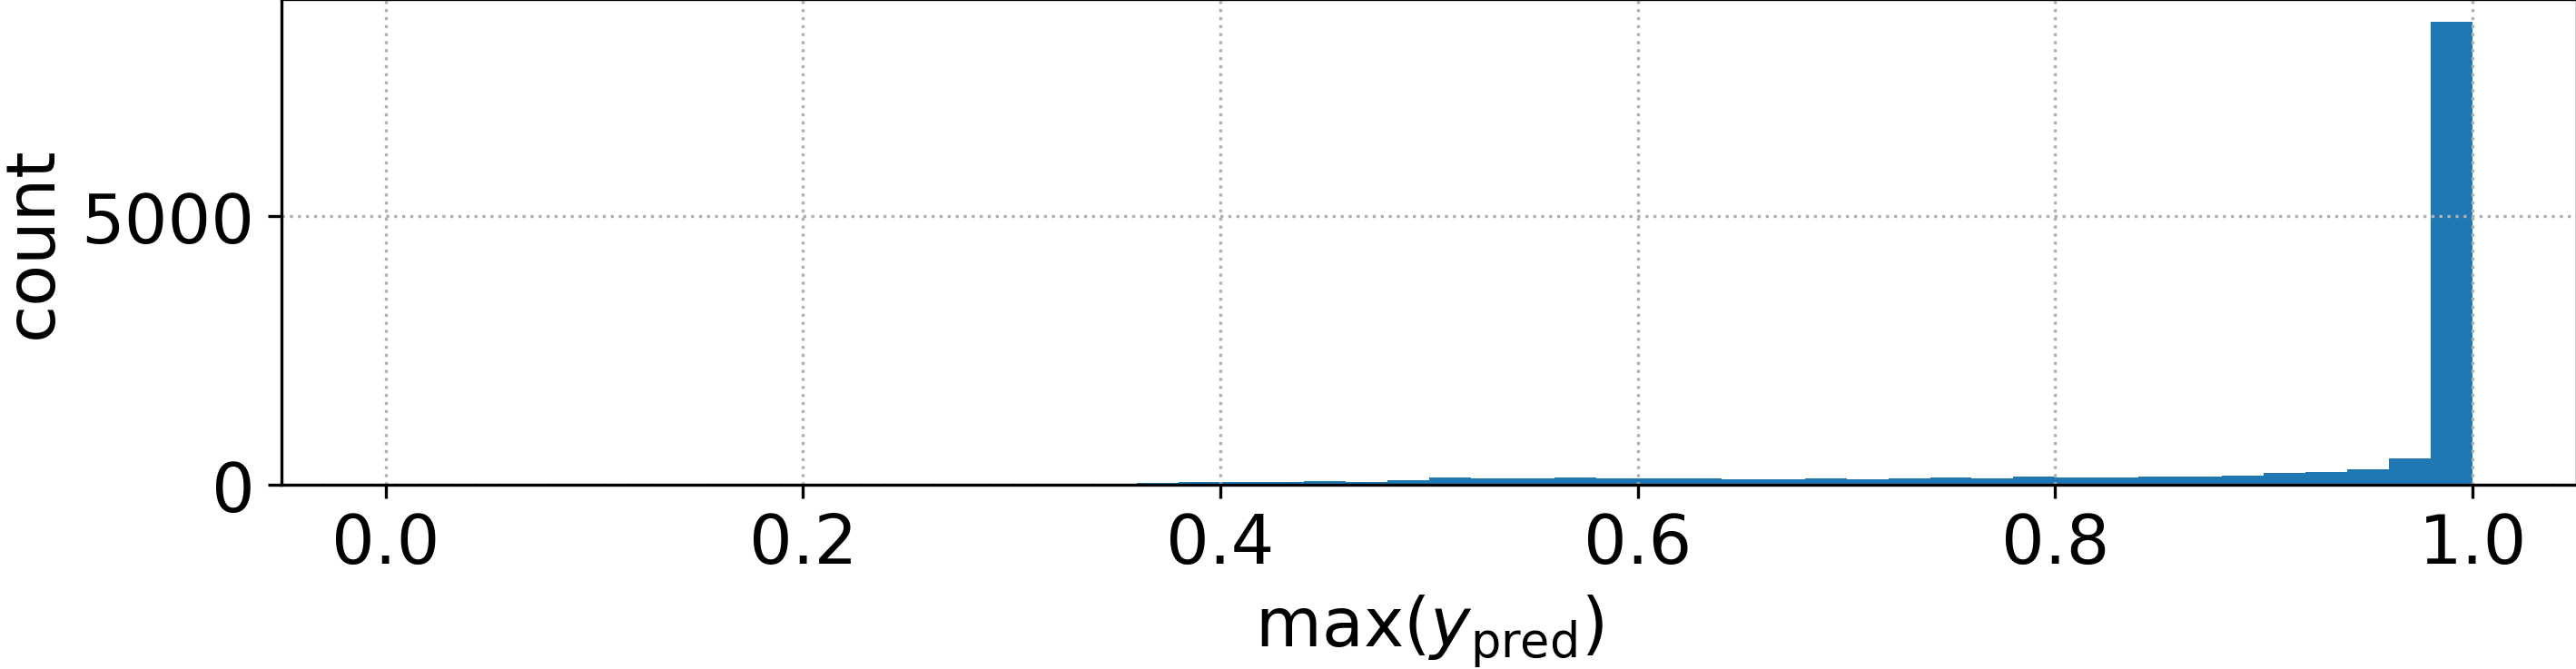
\includegraphics[width=0.8\textwidth]{figures/v1_real/vit_model_V1_original_redomax_ypred_binary_31.png}
        \caption{Spectral ViT V1 Maximum Output Vector Value\label{fig:v1_max}}
    \end{figure}
\end{frame}

\begin{frame}{Spectral ViT V1 Cuts}
    \begin{figure}[b]
        \centering
        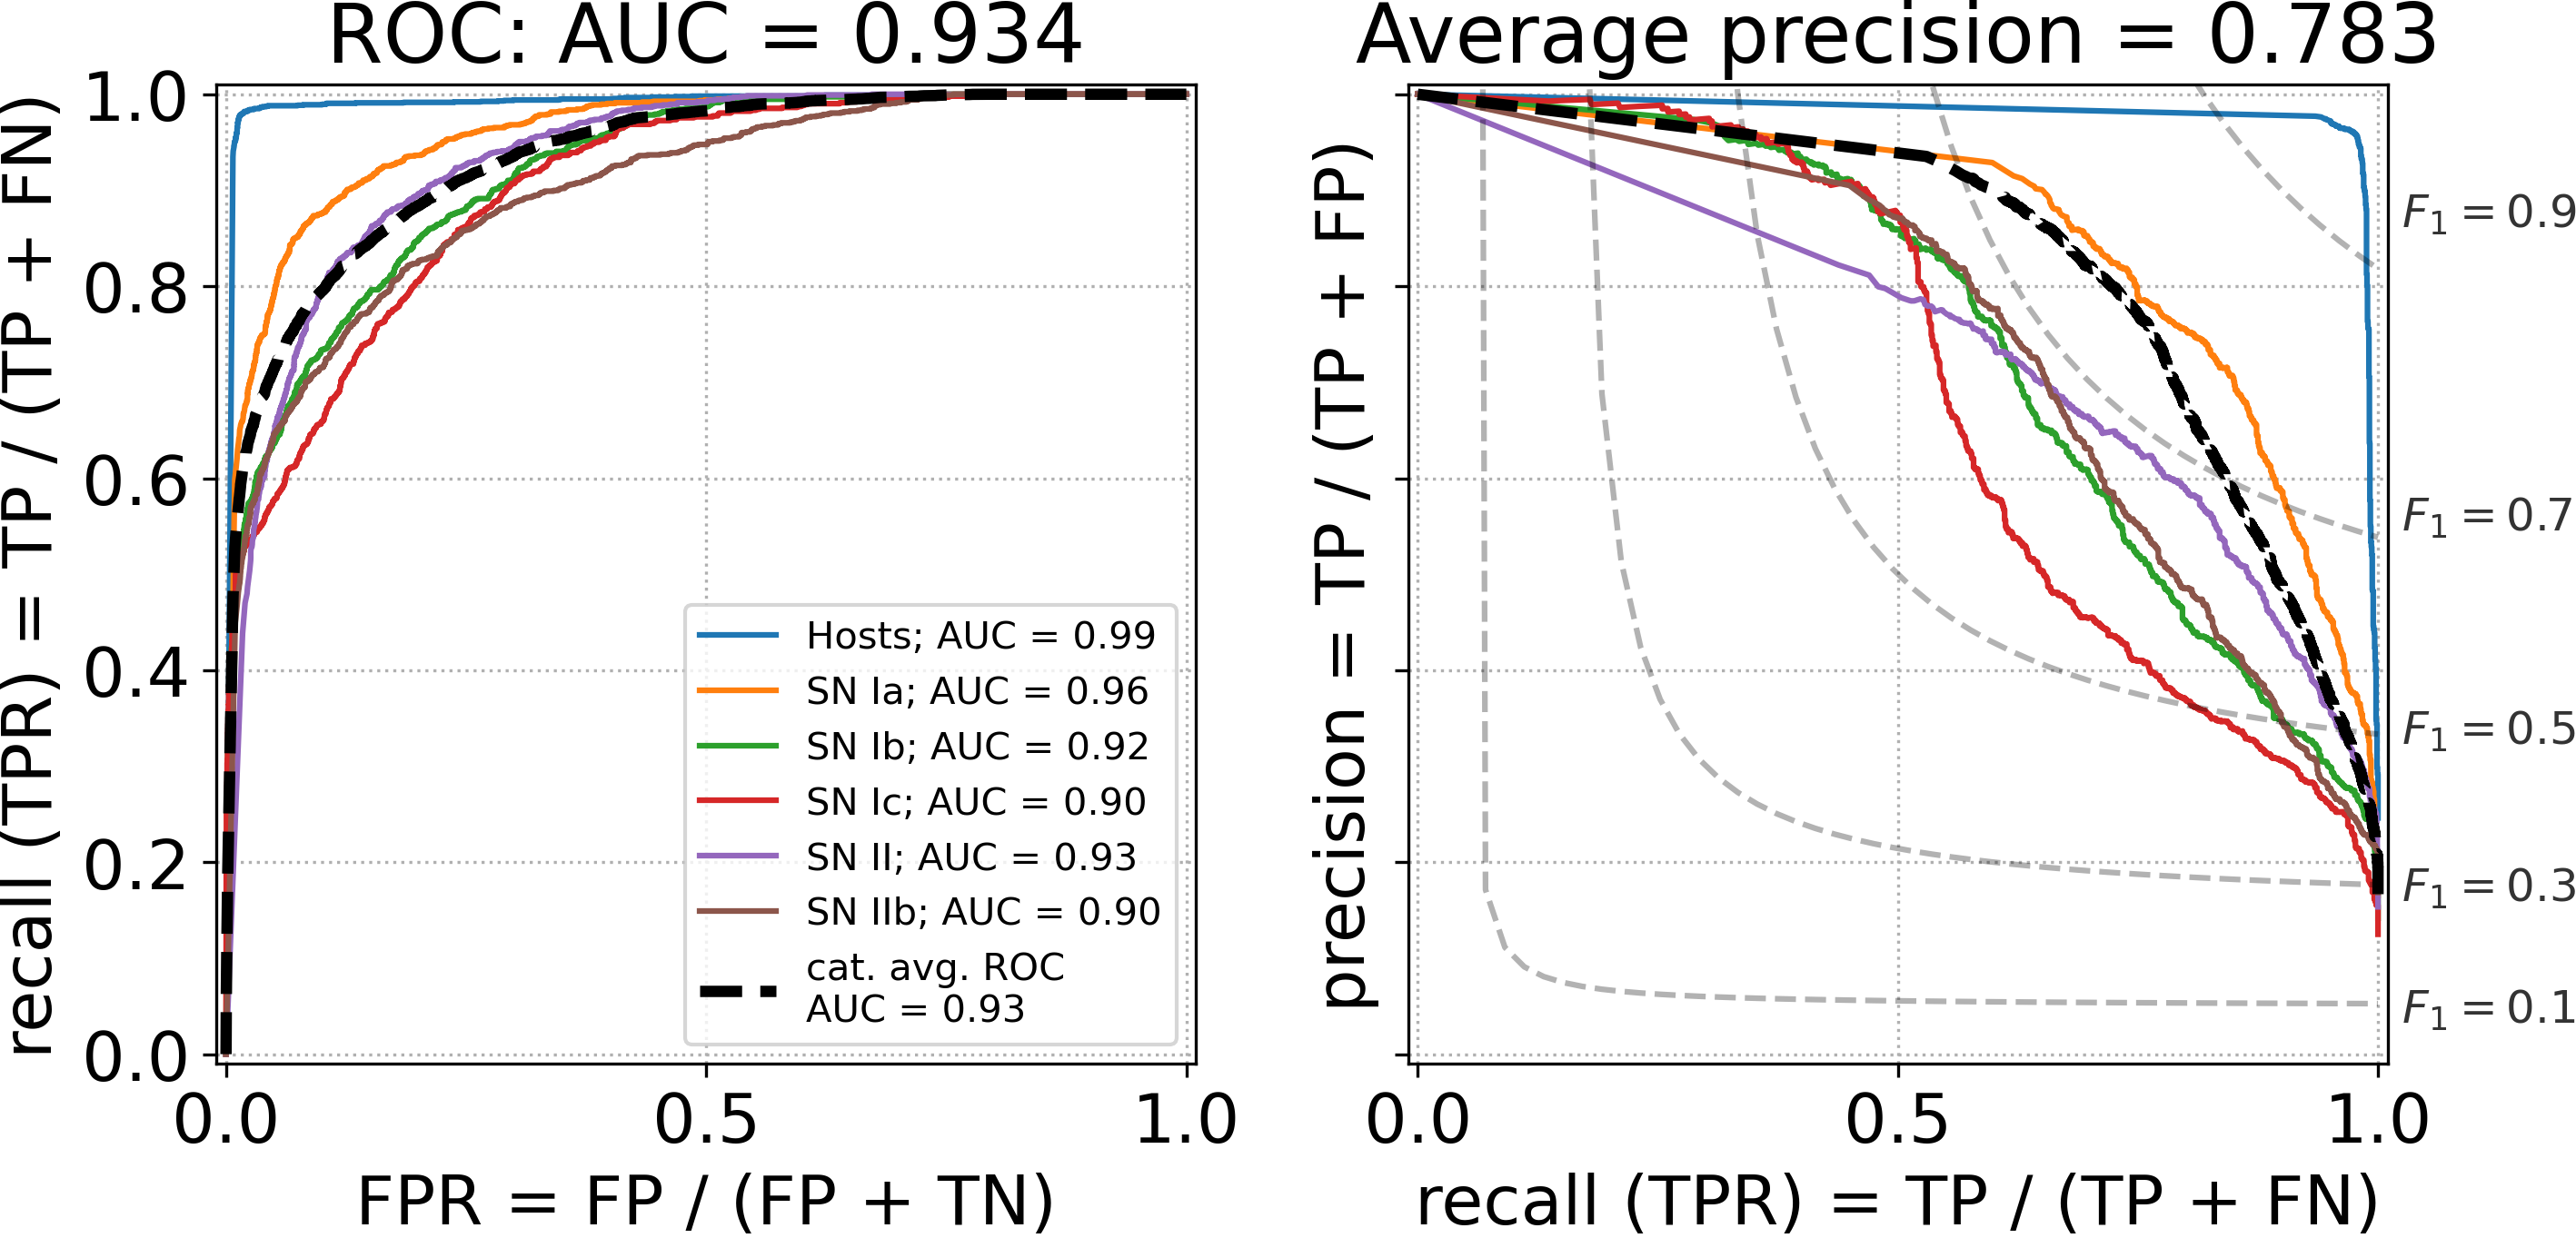
\includegraphics[height=2.6cm]{figures/v1_real/vit_model_V1_original_redoroc99_e31.png}
        \quad
        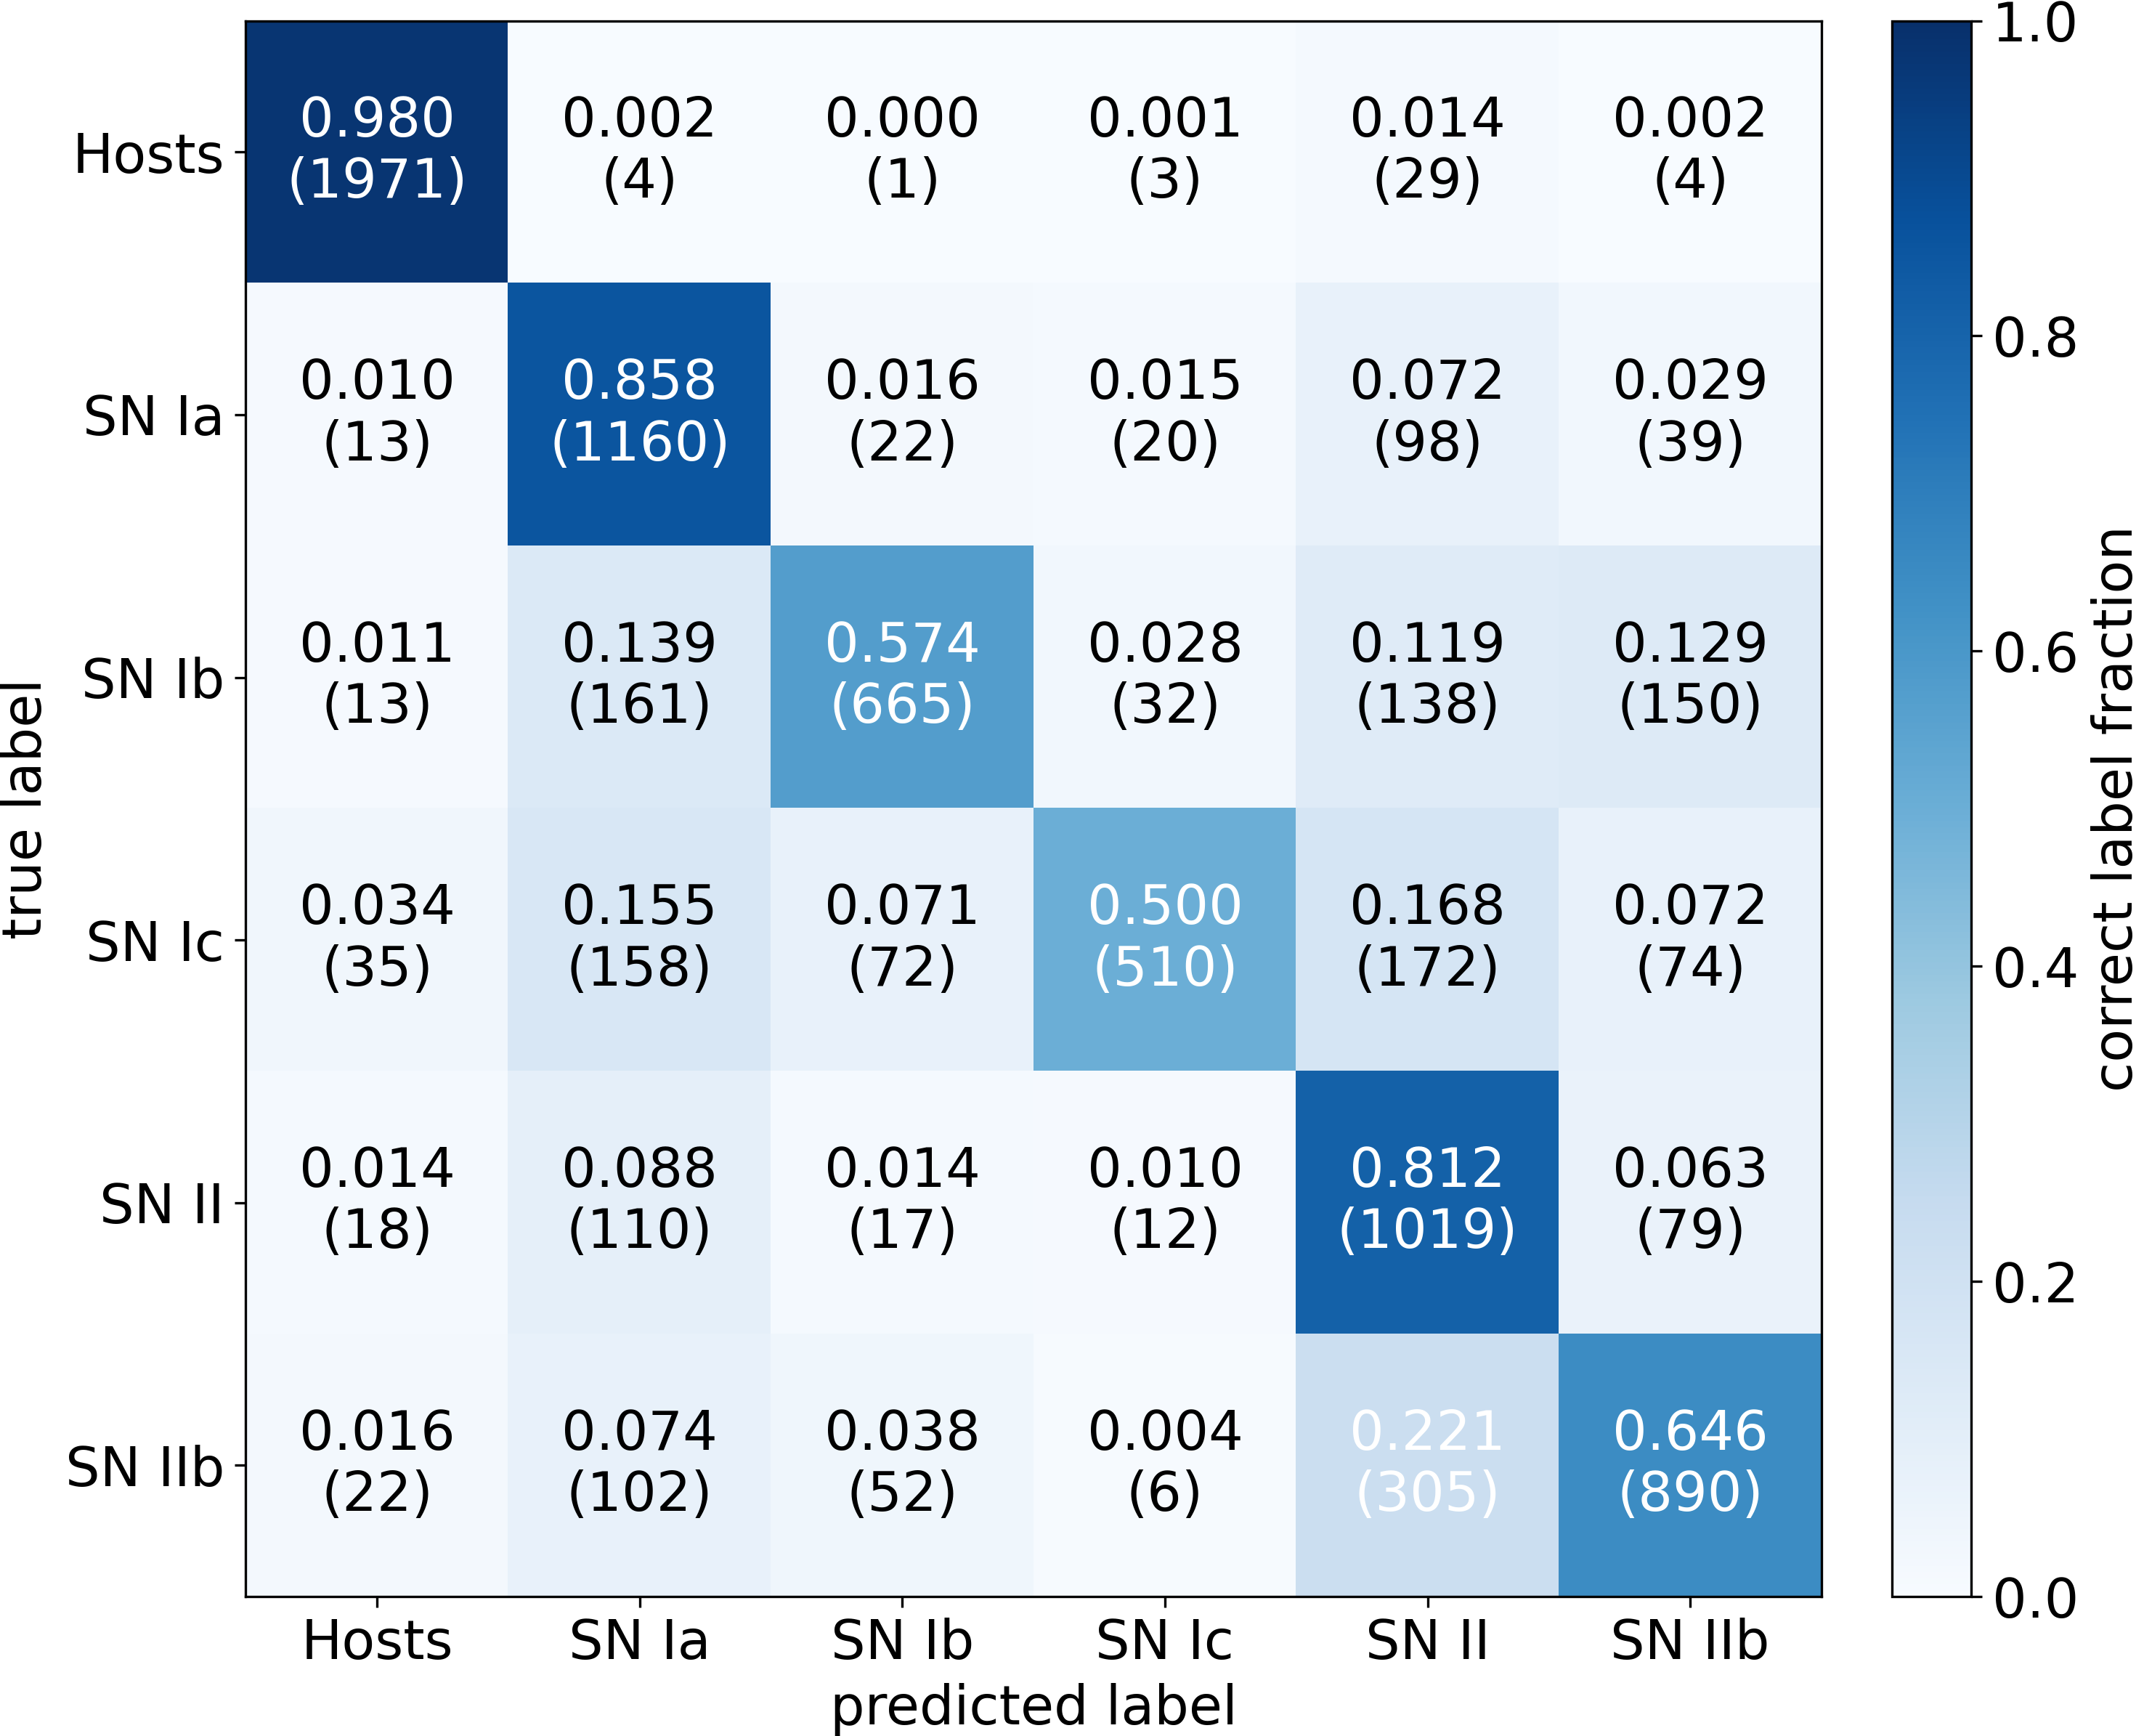
\includegraphics[height=2.6cm]{figures/v1_real/vit_model_V1_original_redocm99_e31.png}
        \caption{Spectral ViT V1 Classifier: 99\% confidence cut \label{fig:v1_99_qual}}
        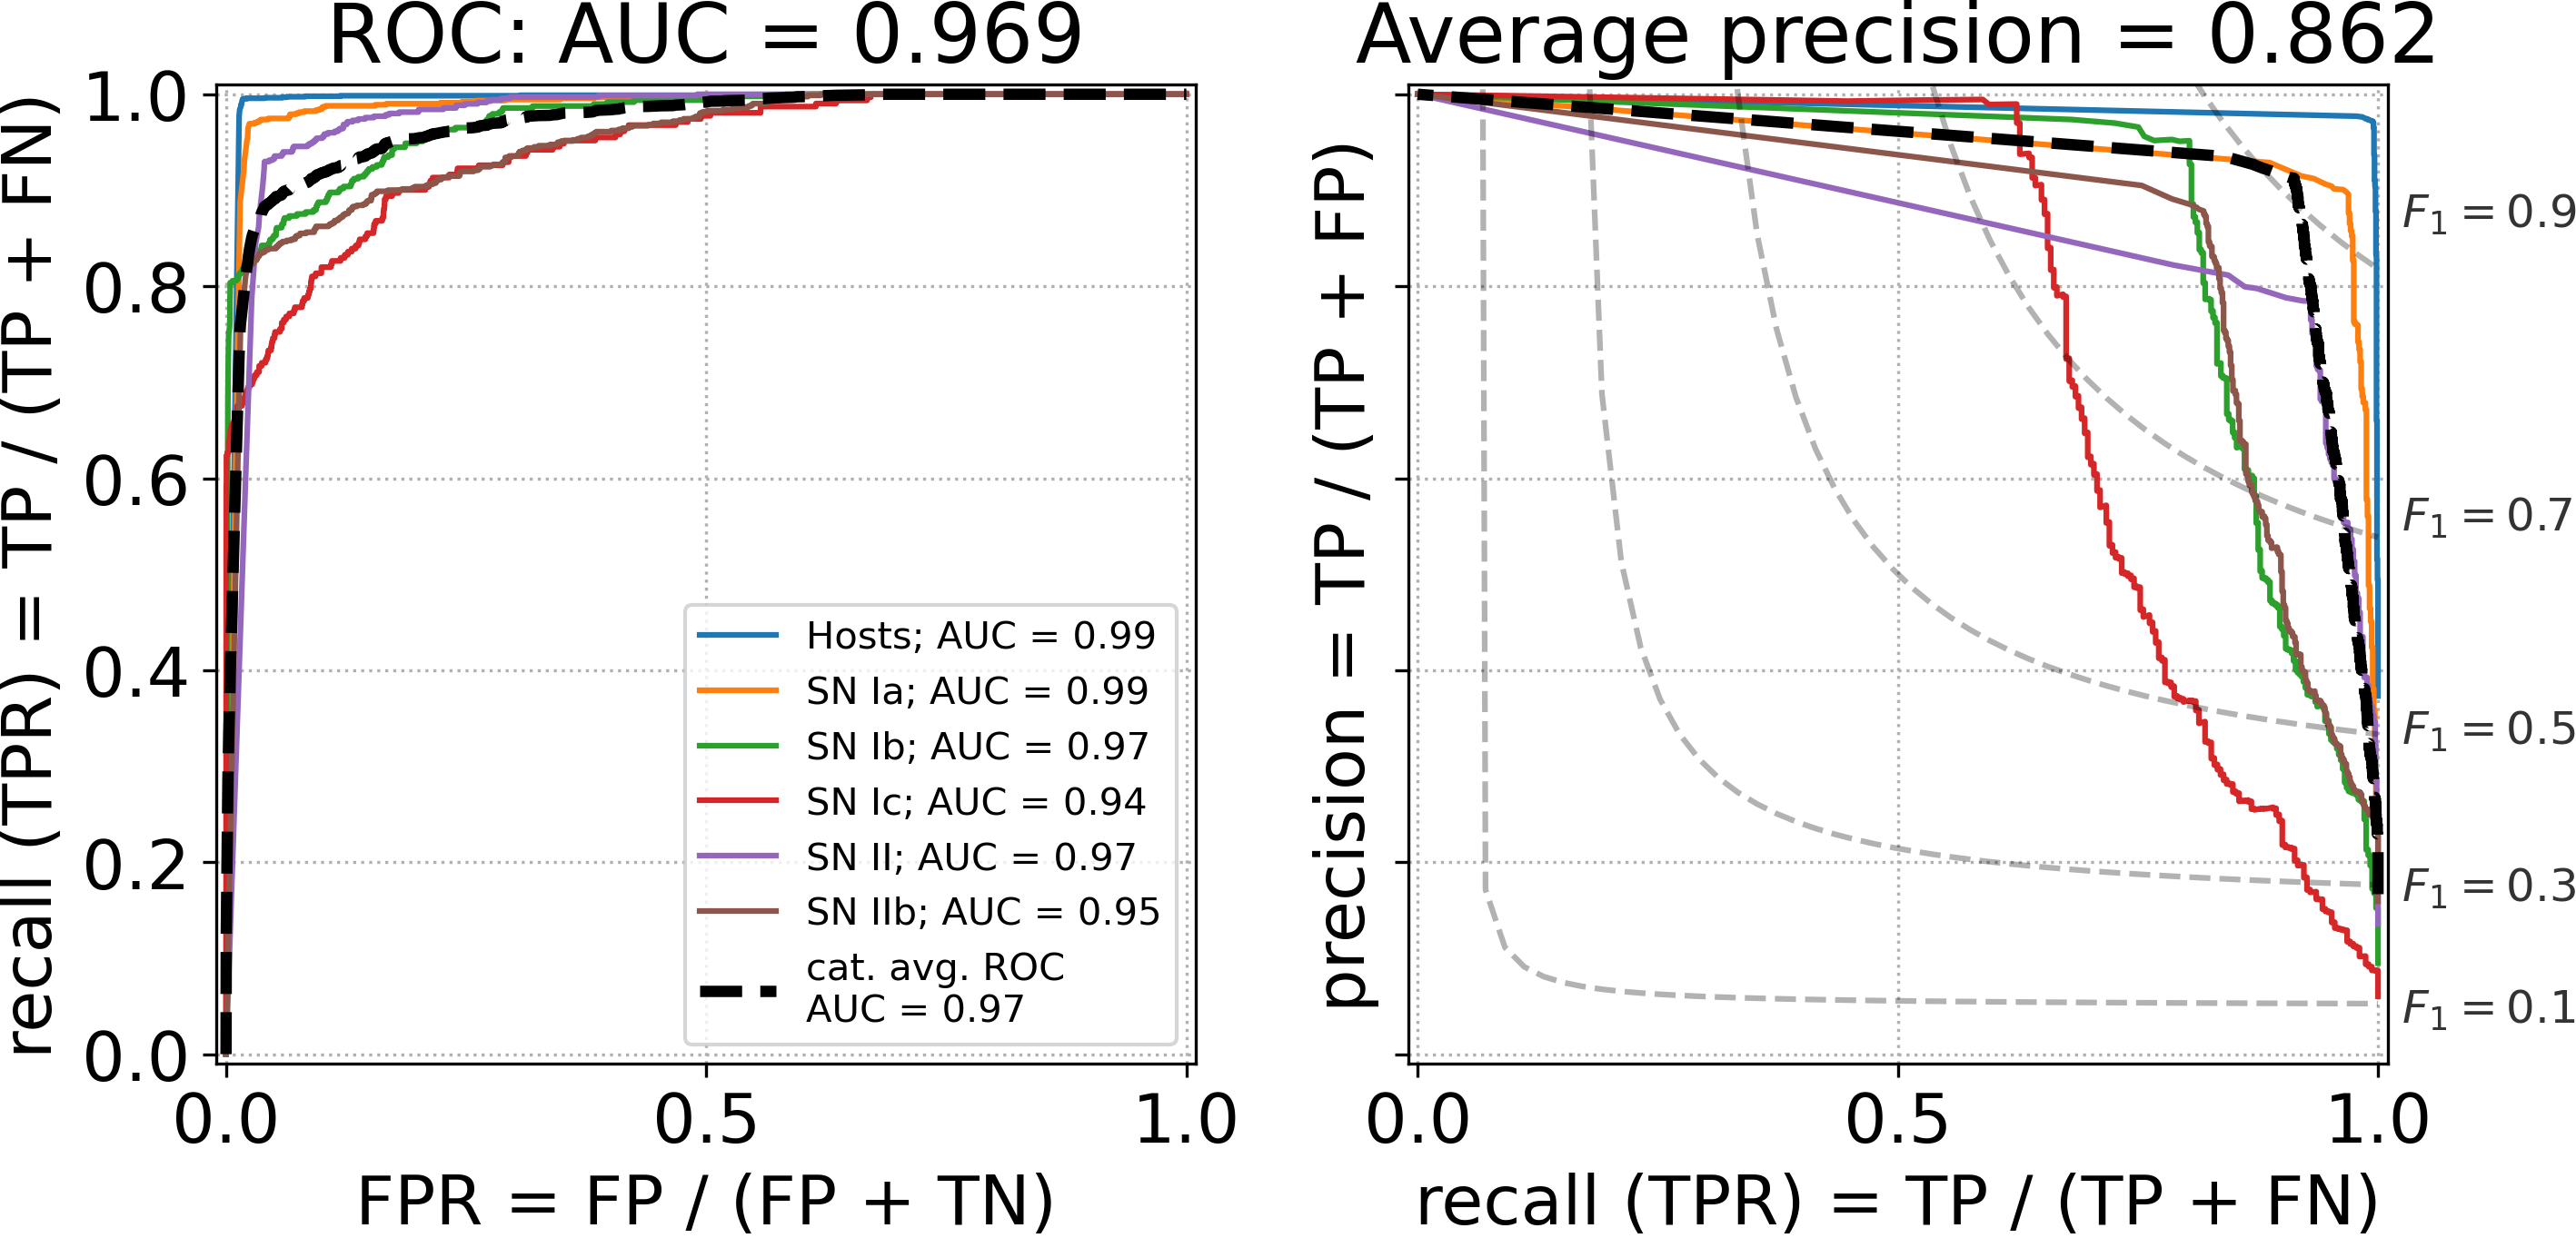
\includegraphics[height=2.6cm]{figures/v1_real/vit_model_V1_original_redoroc999999_e31.png}
        \quad
        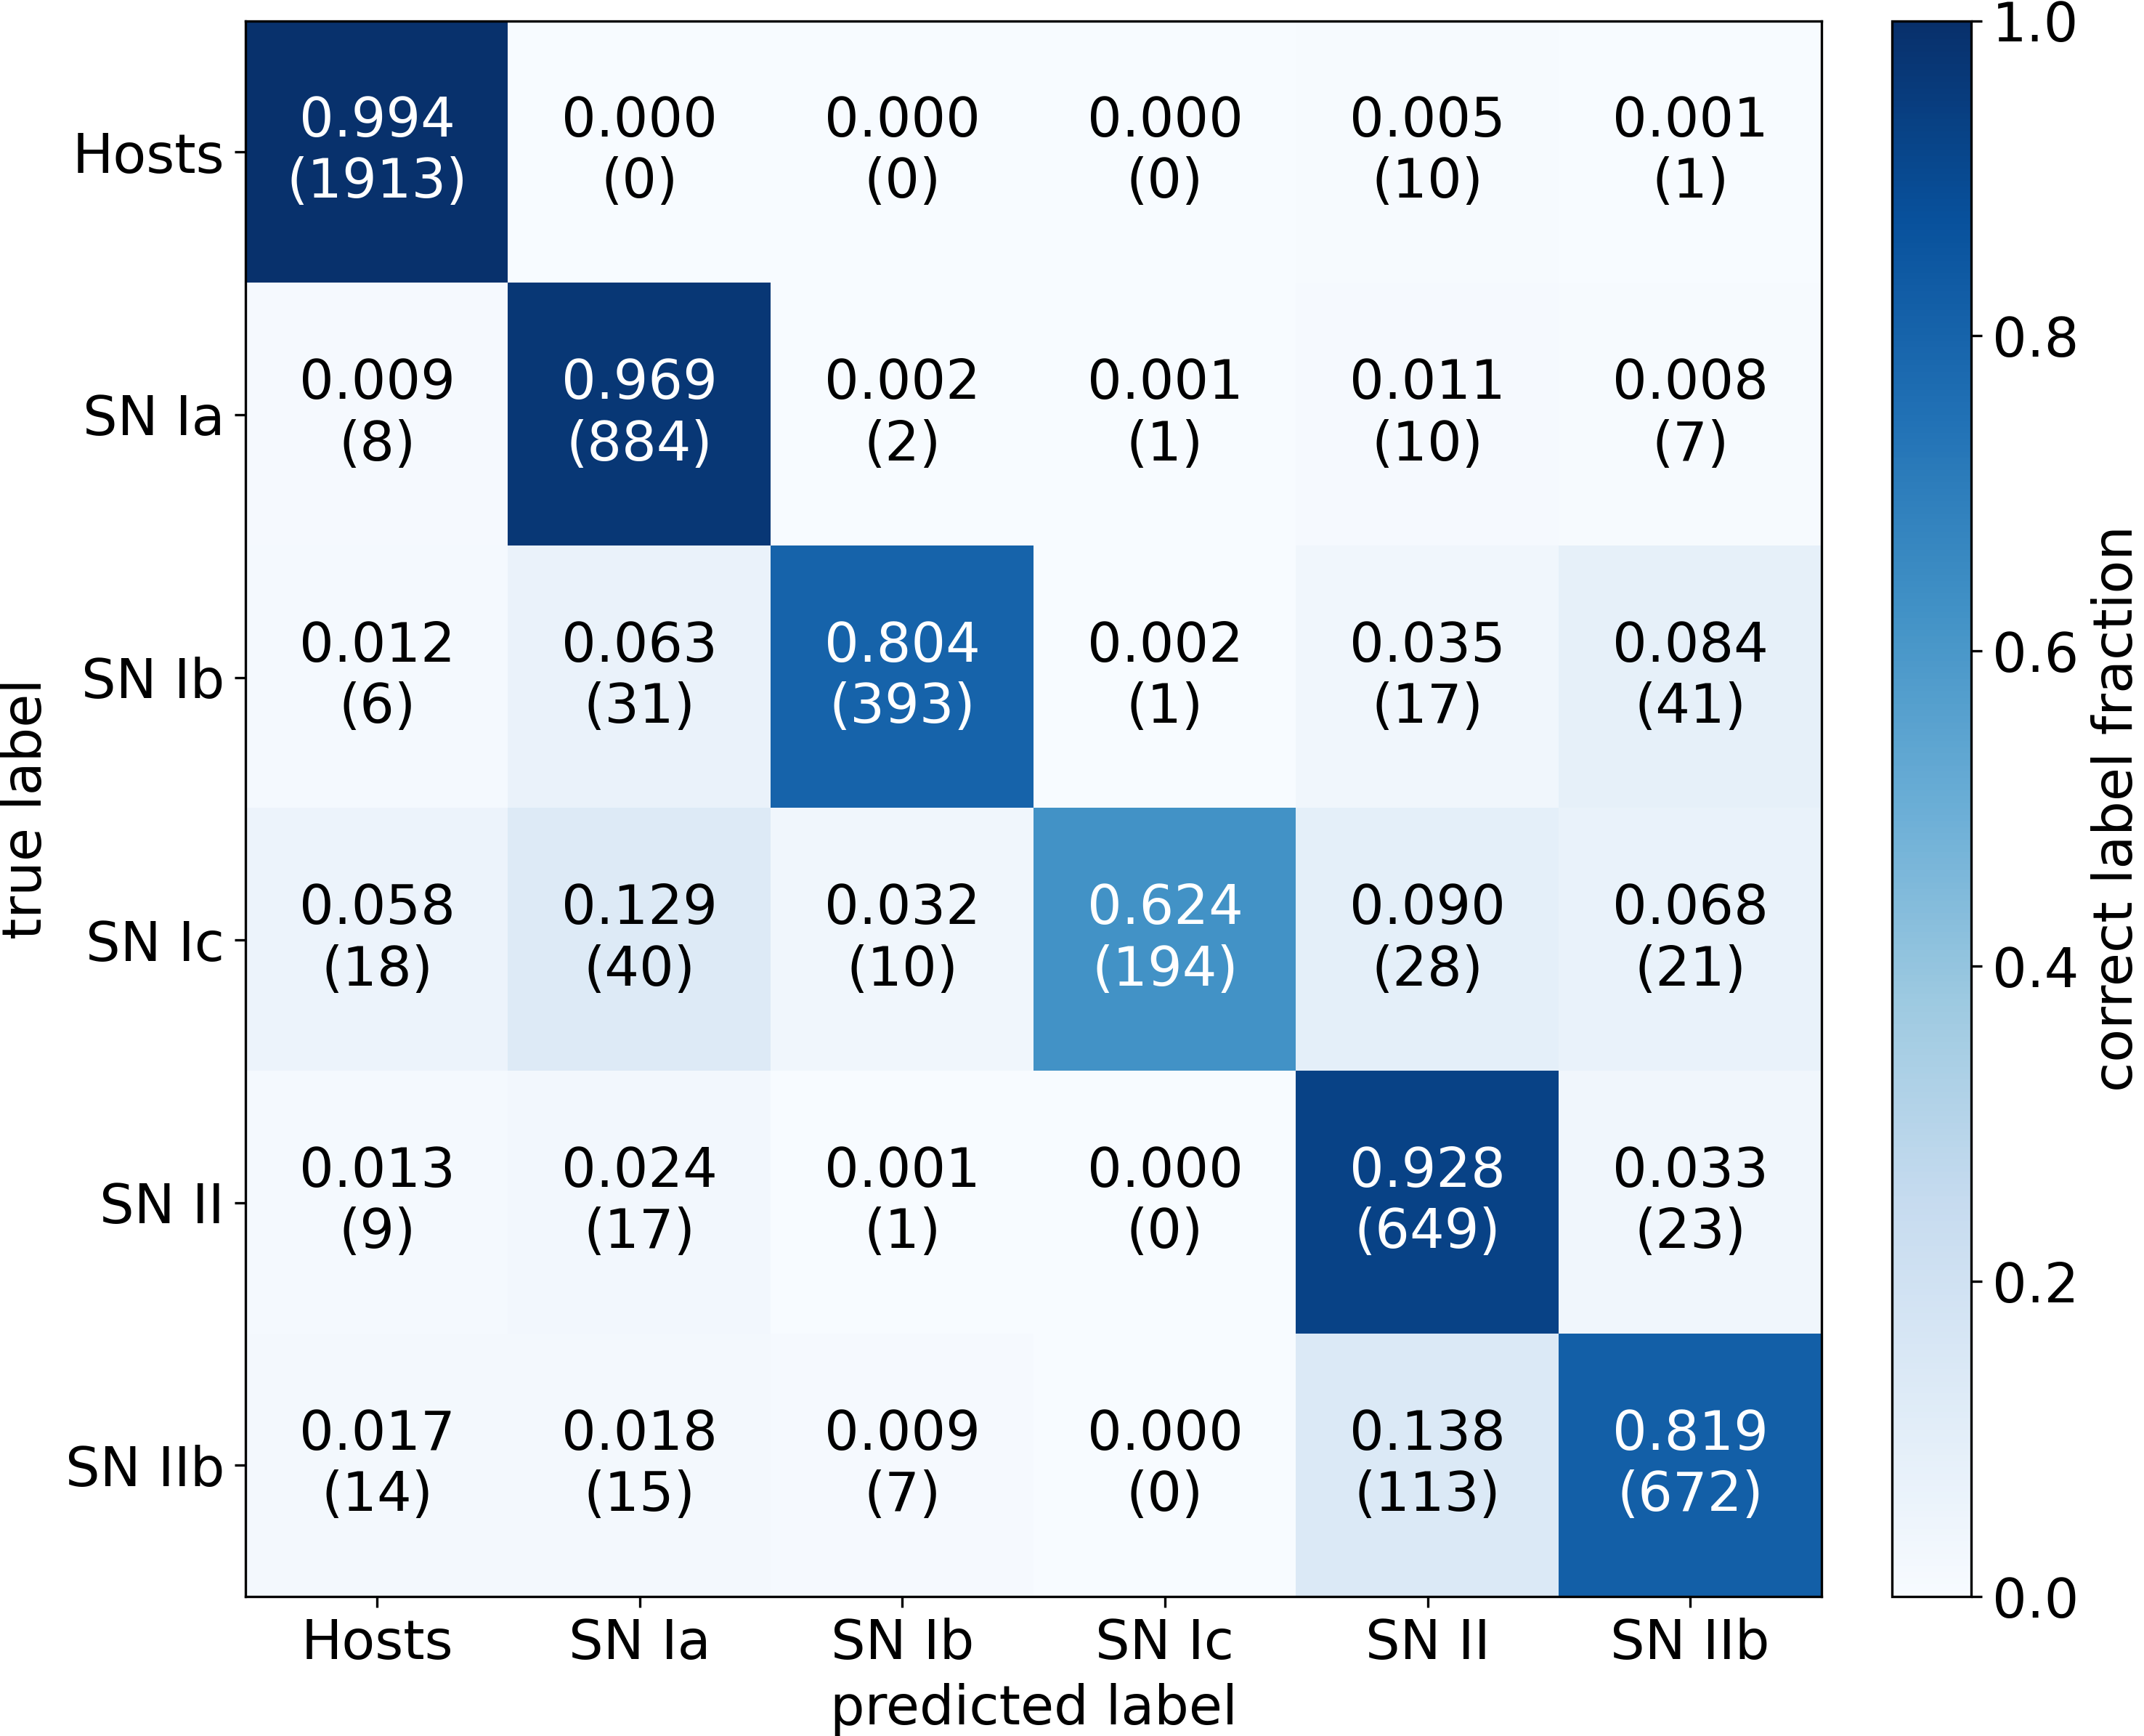
\includegraphics[height=2.6cm]{figures/v1_real/vit_model_V1_original_redocm999999_e31.png}
        \caption{Spectral ViT V1 Classifier: 99.9999\% confidence cut \label{fig:v1_999999_qual}}
    \end{figure}
\end{frame}

% \section{Spectral ViT V2: Specialized Classifier}
\begin{frame}
    \begin{figure}[b!]
        \centering
        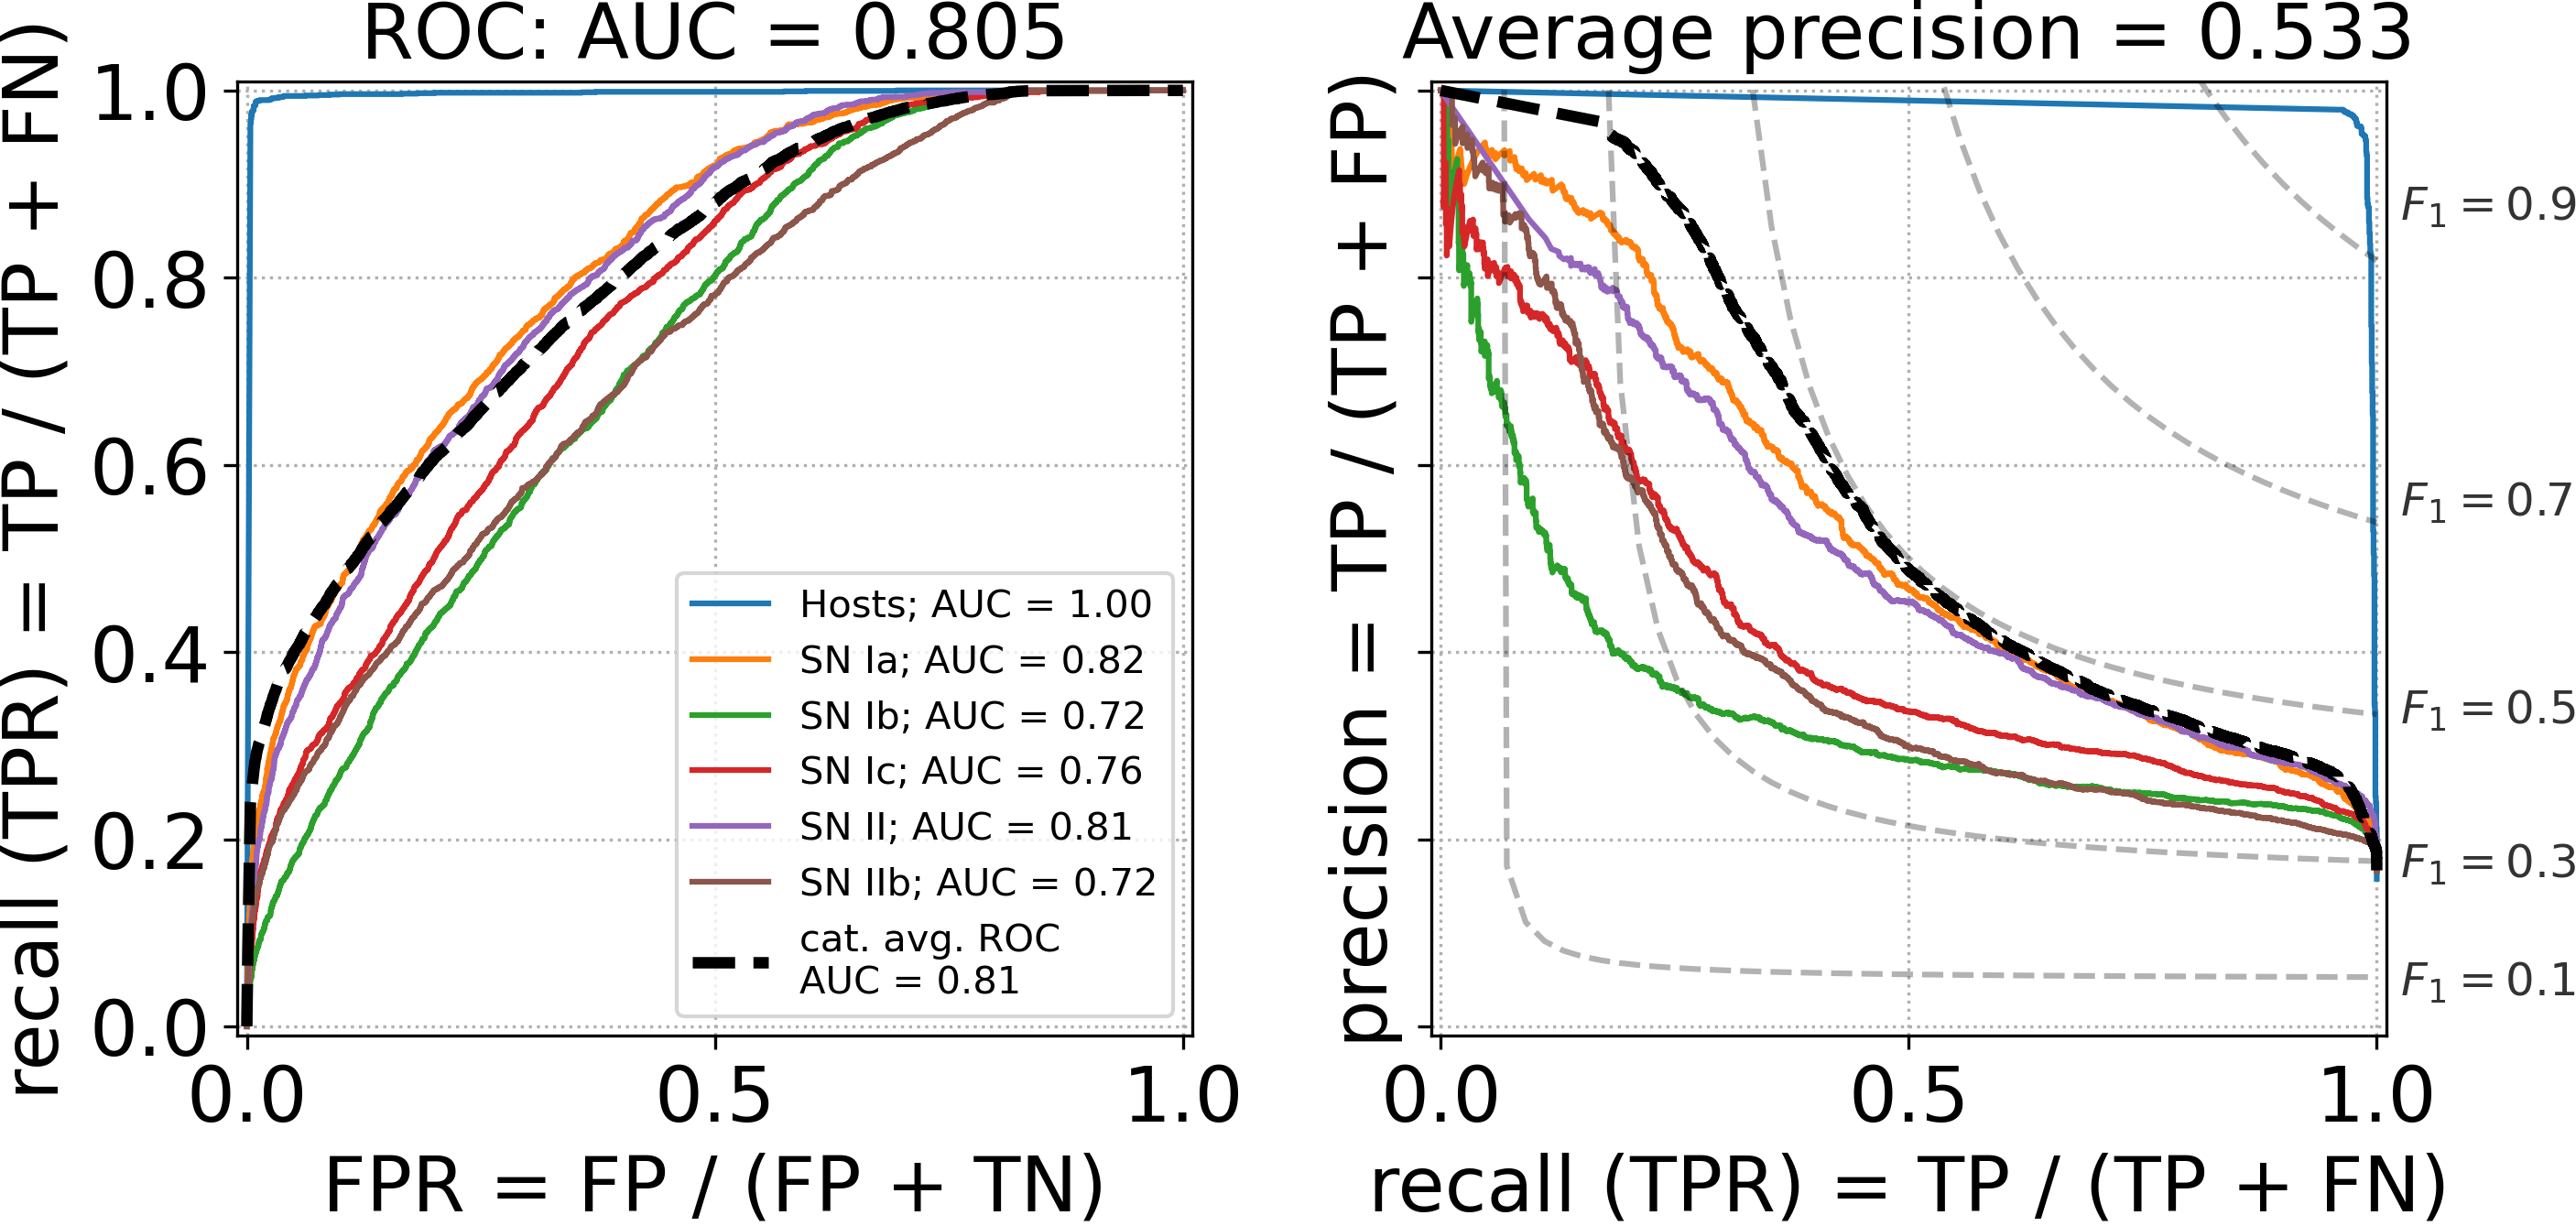
\includegraphics[height=2.8cm]{figures/v2_real/vit_model_V2rocfulle_e26.png}
        \quad
        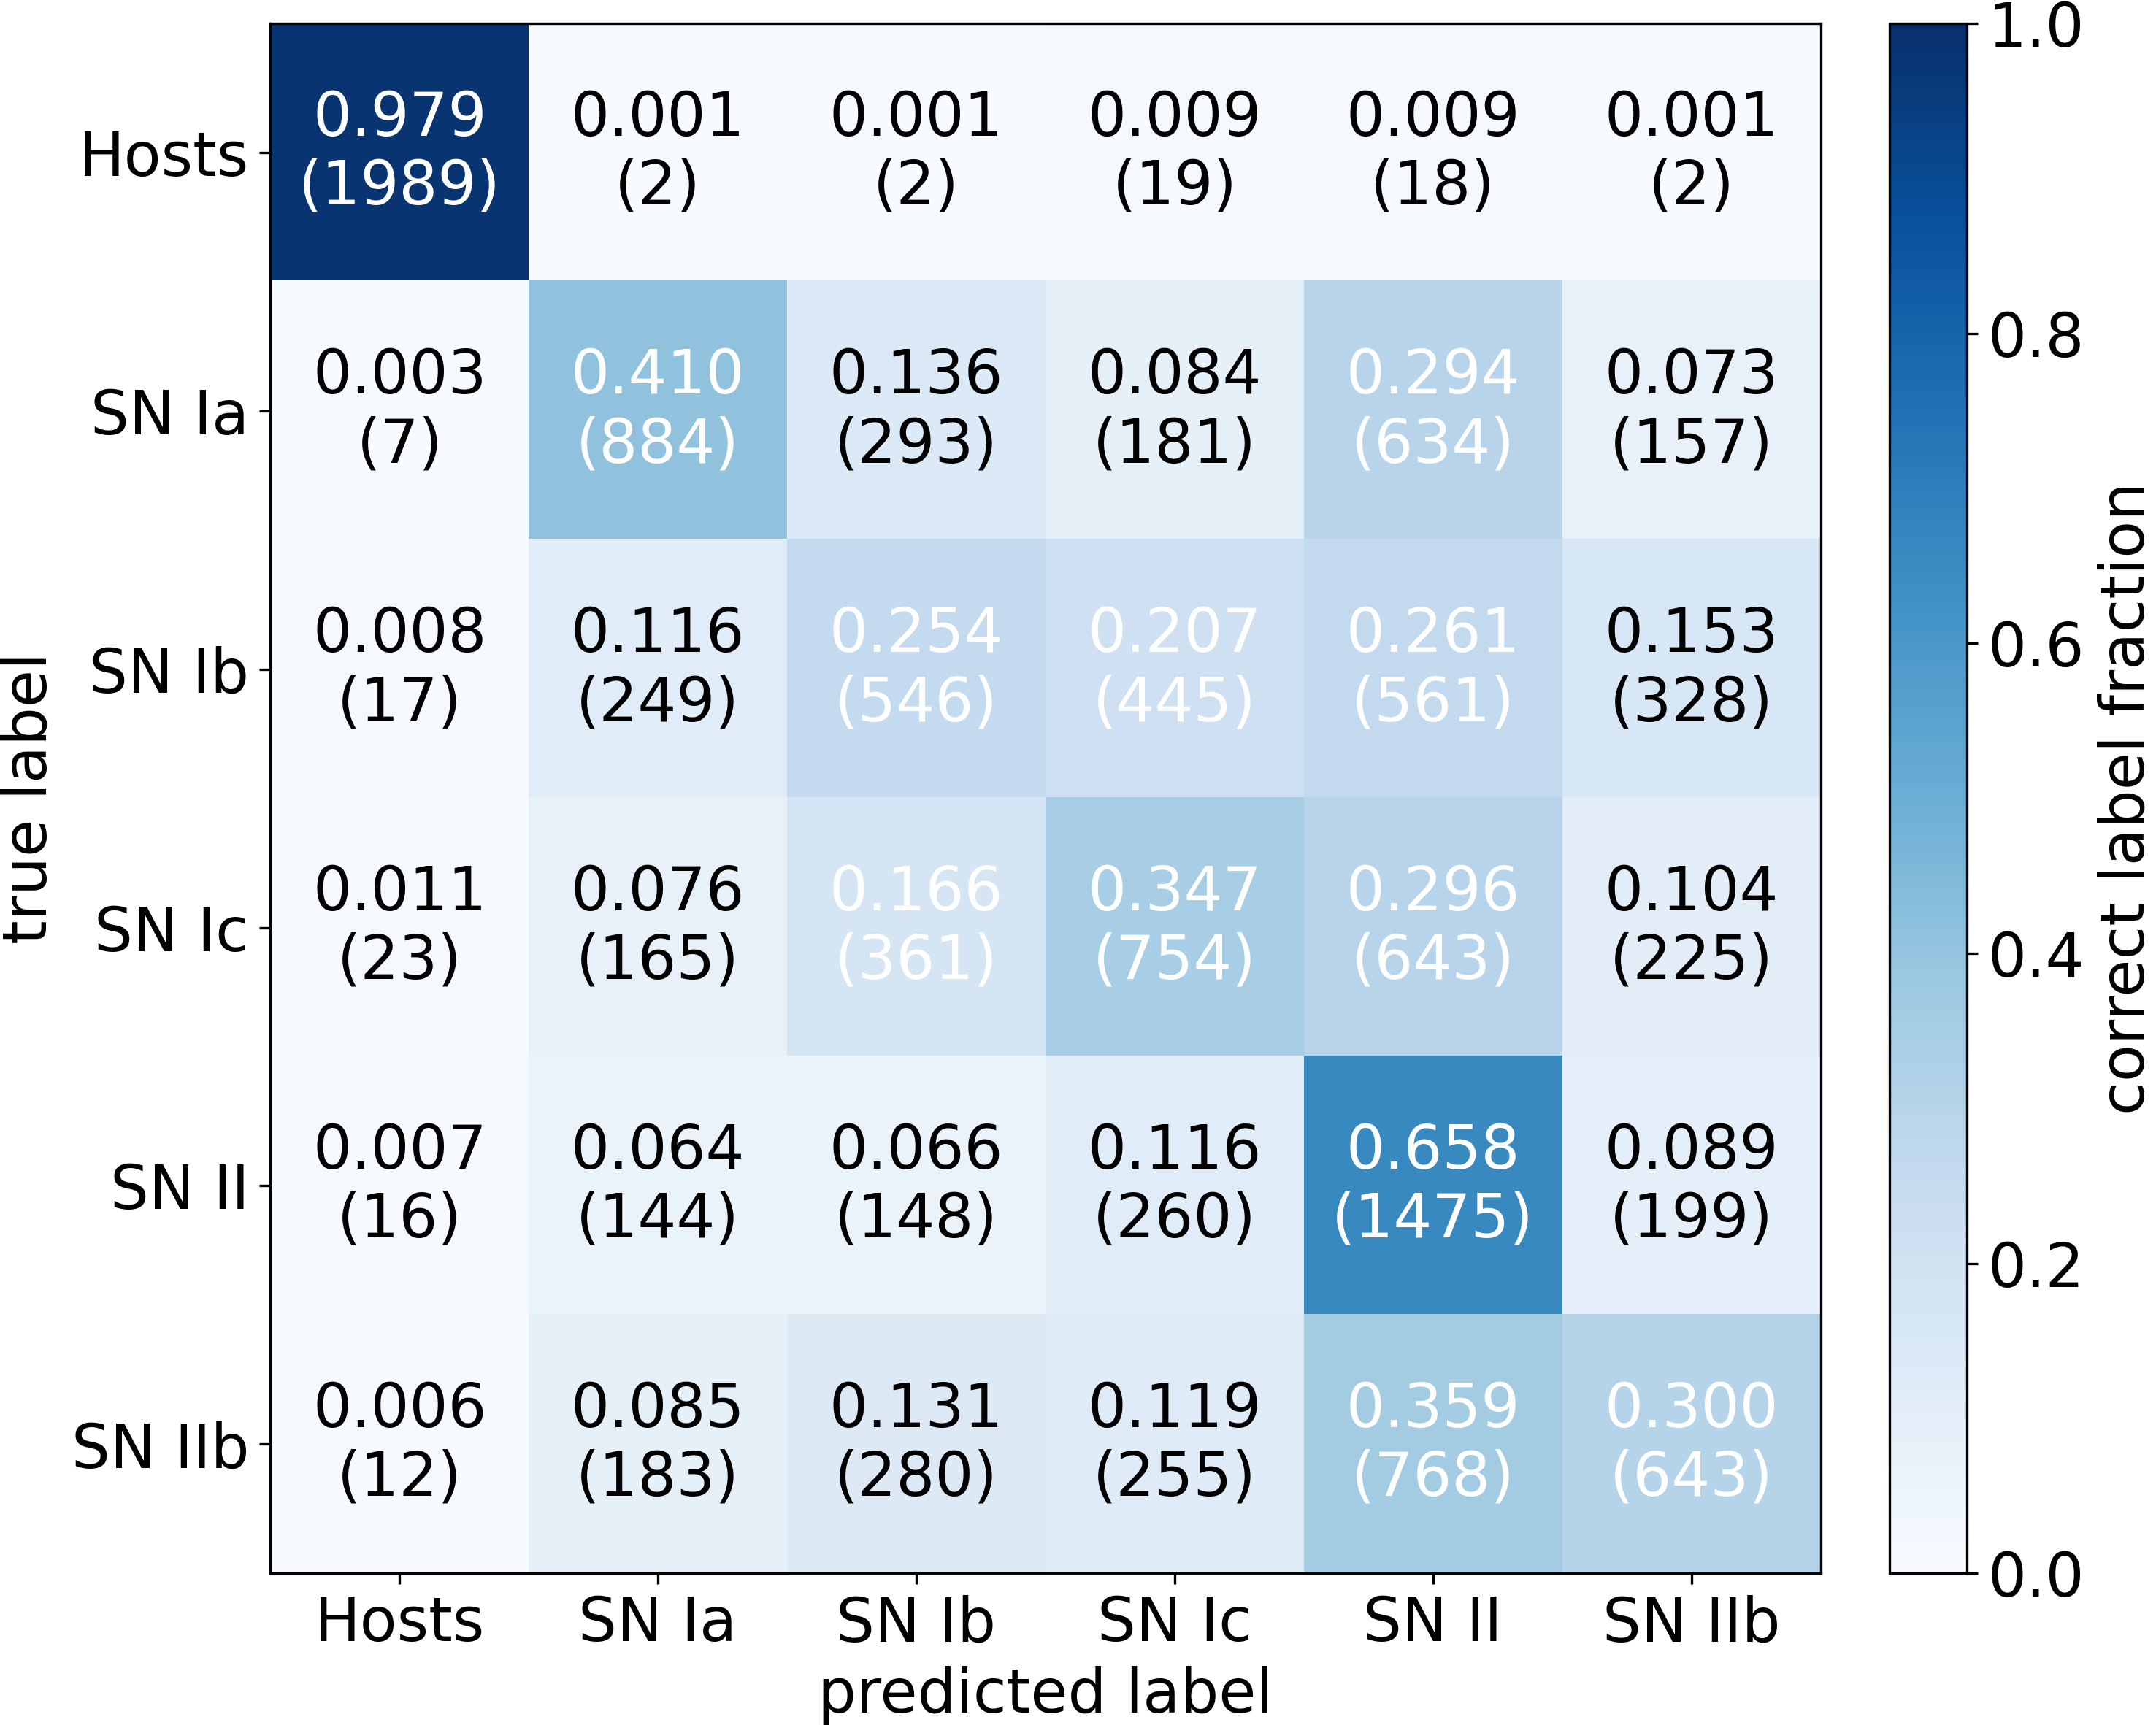
\includegraphics[height=2.8cm]{figures/v2_real/vit_model_V2cmfull_e26.png}
        \caption{Spectral ViT V2 Classifier\label{fig:v2_qual}}
%     \end{figure}
% \end{frame}

% \begin{frame}
%     \begin{figure}[t!]
%         \centering
        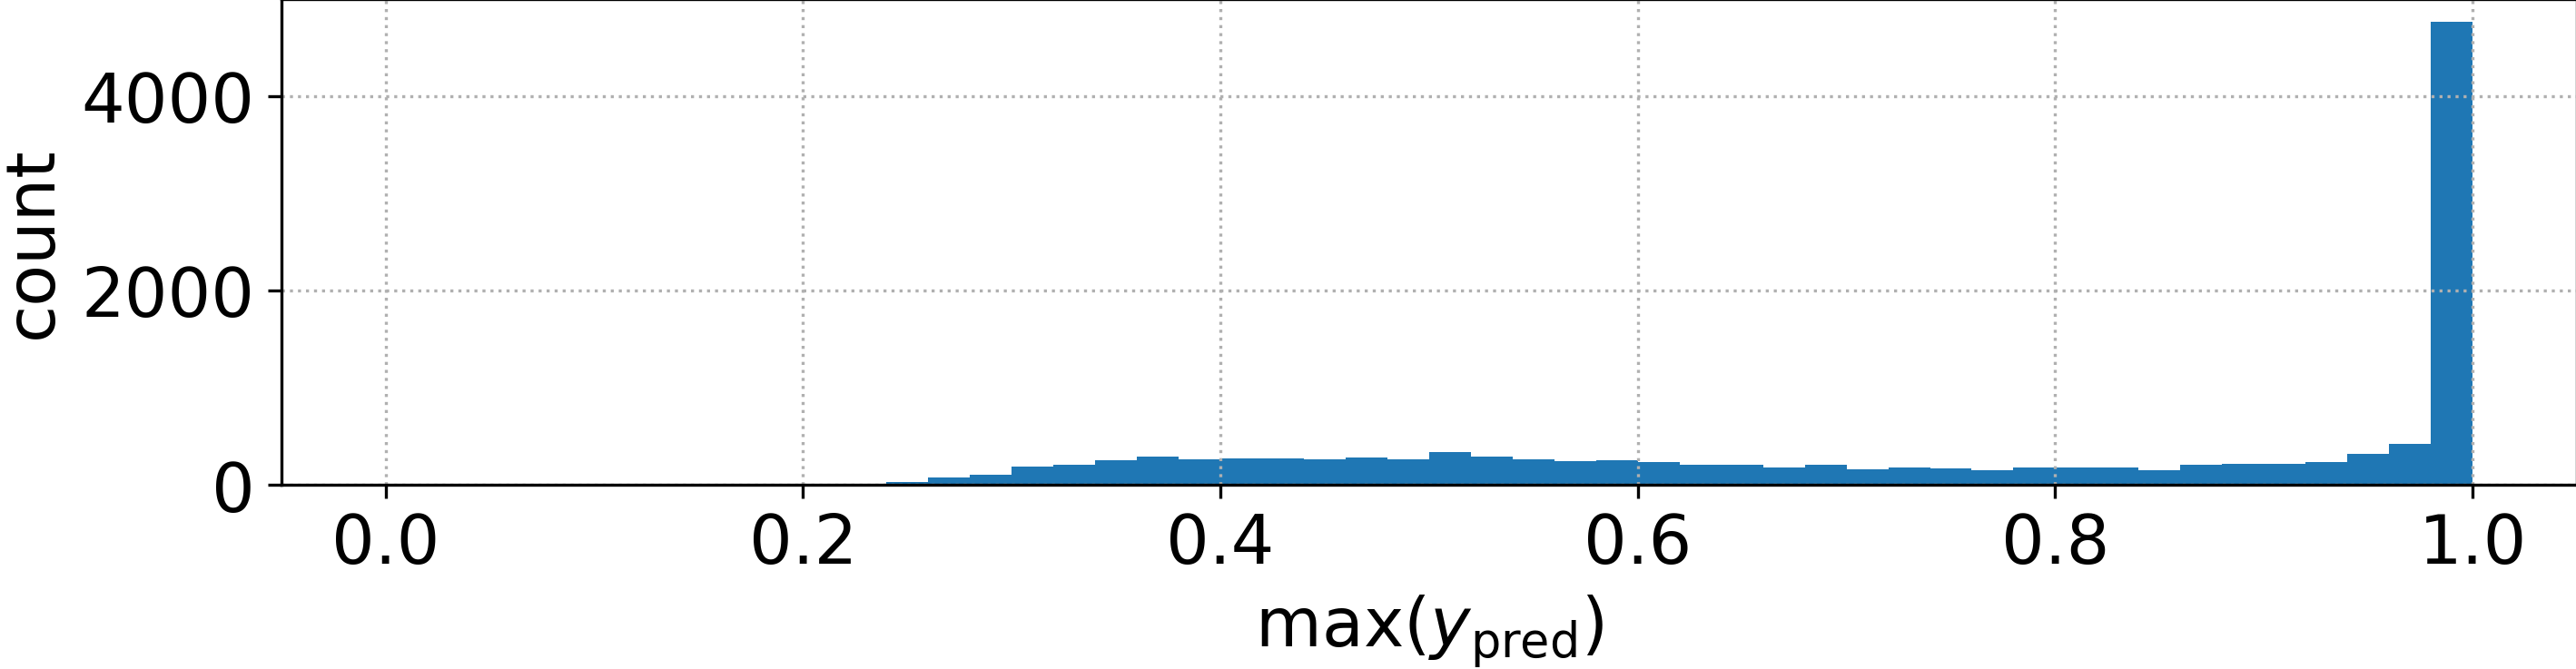
\includegraphics[width=0.8\textwidth]{figures/v2_real/vit_model_V2max_ypred_26.png}
        \caption{Spectral ViT V2 Maximum Output Vector Value\label{fig:v2_max}}
    \end{figure}
\end{frame}

\begin{frame}
    \begin{figure}[b!]
        \centering
        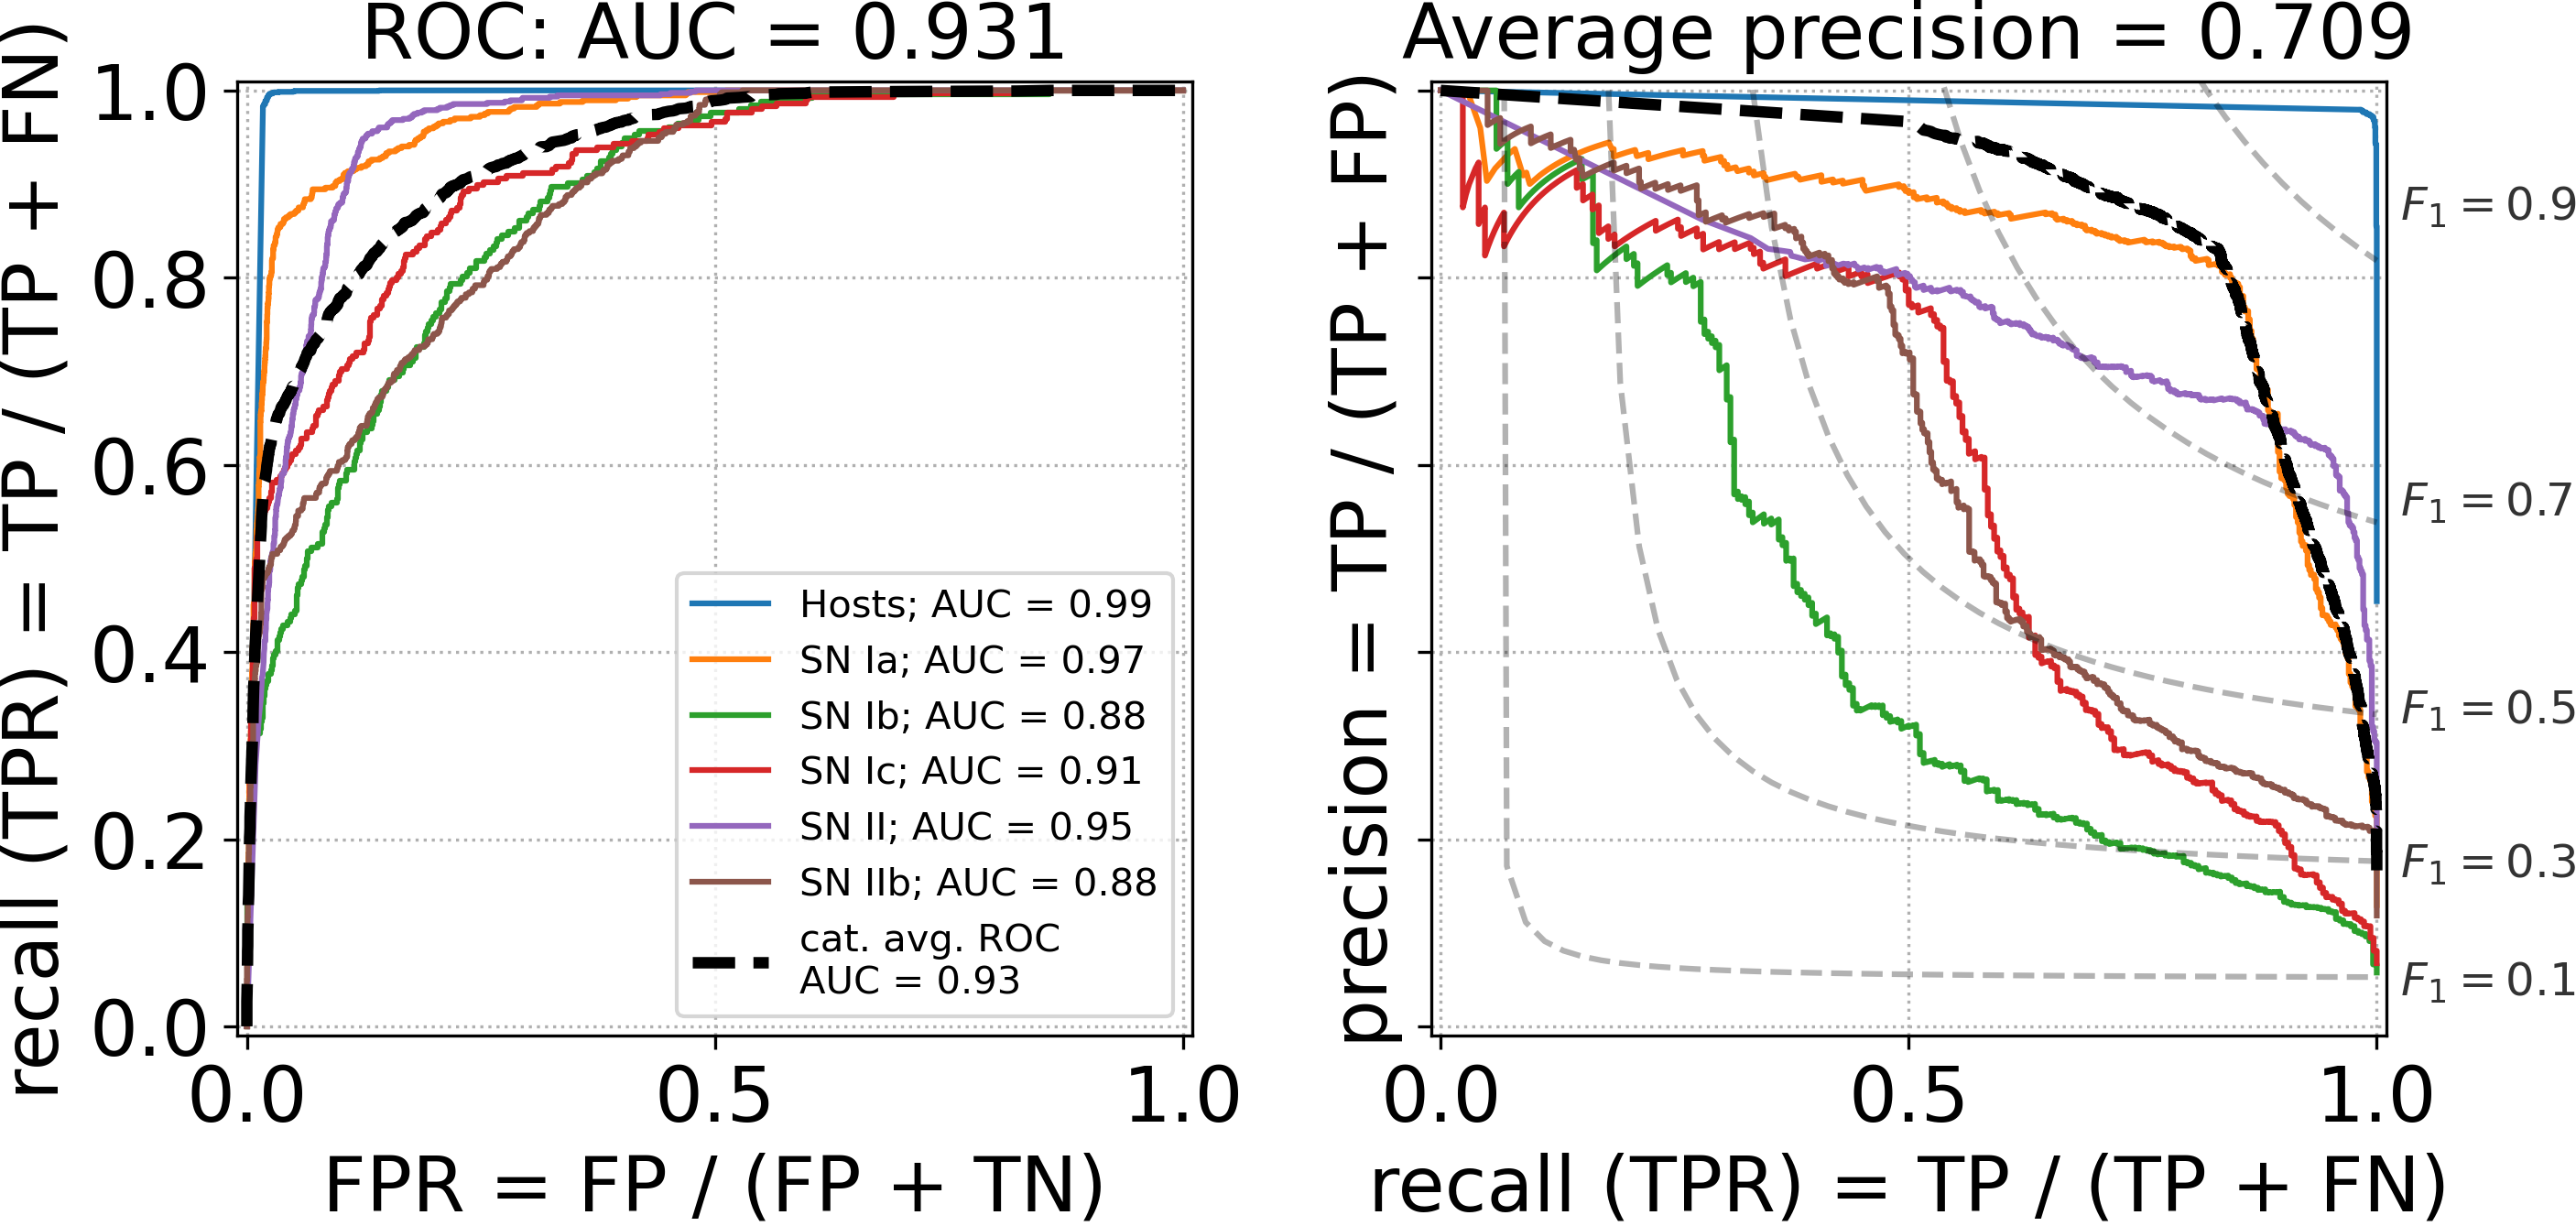
\includegraphics[height=2.8cm]{figures/v2_real/vit_model_V2roc99_e26.png}
        \quad
        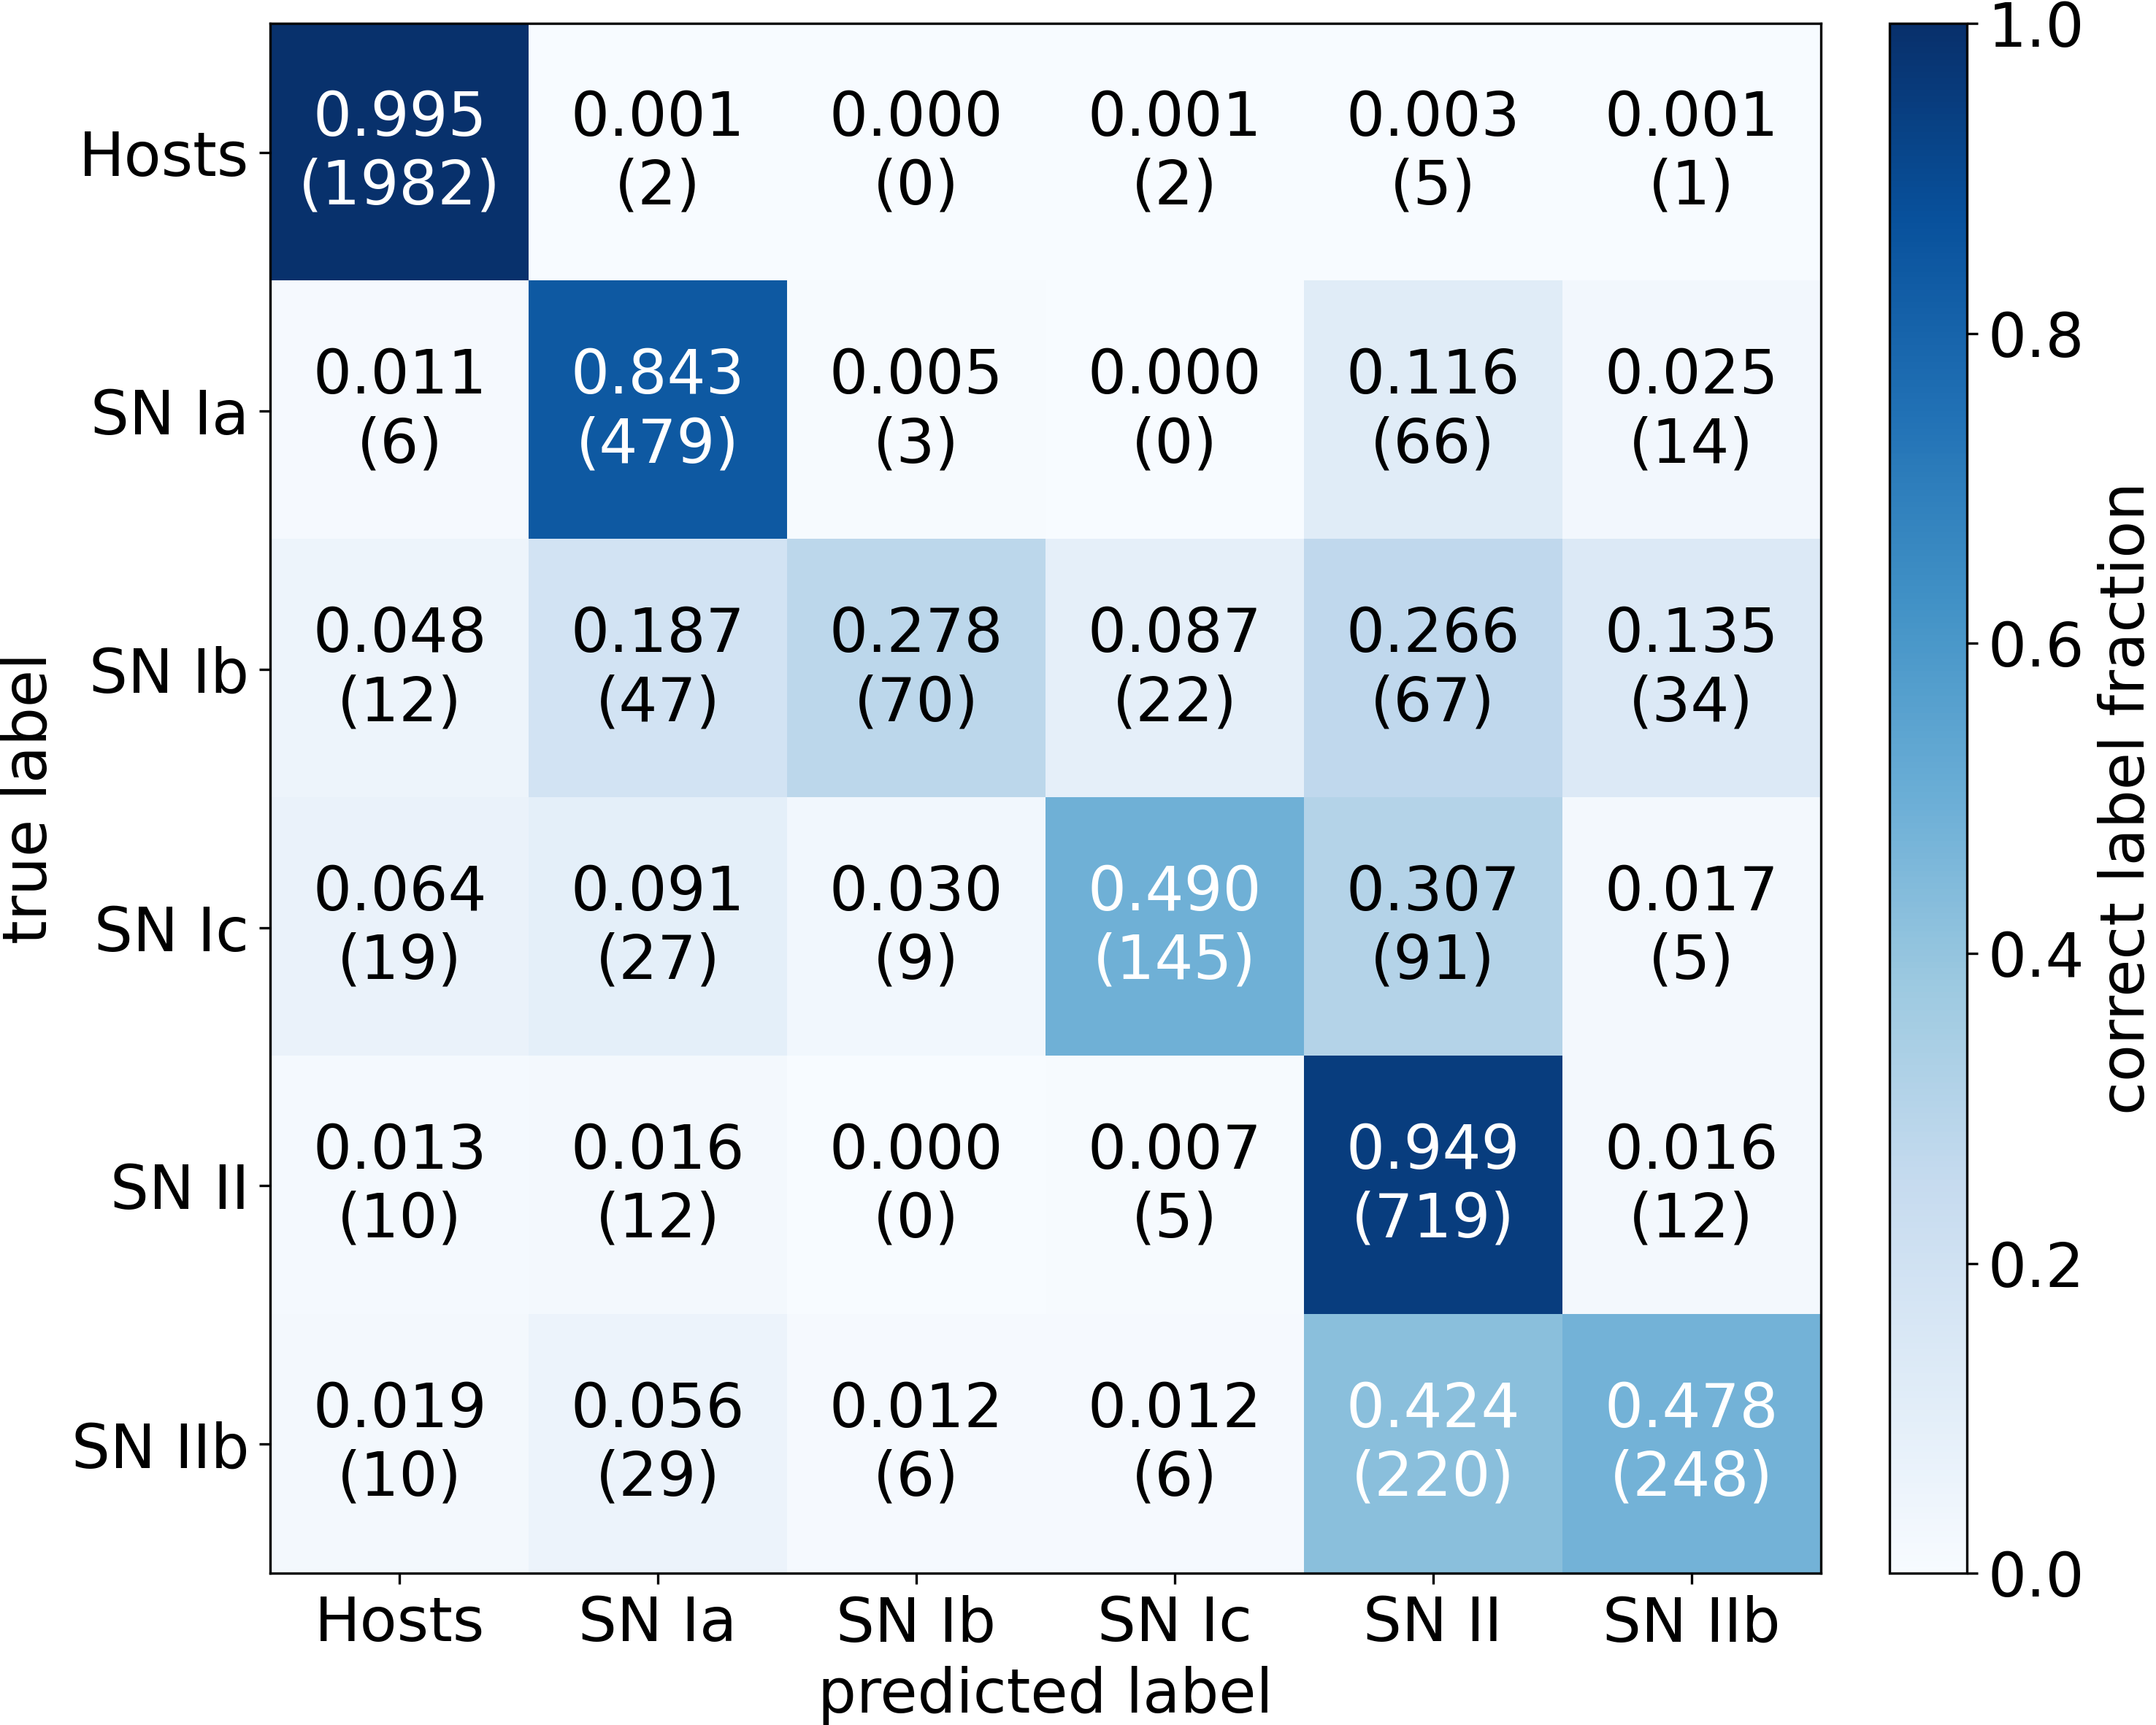
\includegraphics[height=2.8cm]{figures/v2_real/vit_model_V2cm99_e26.png}
        \caption{Spectral ViT V2 Classifier (99\% confidence cut)\label{fig:v2_99_qual}}
    \end{figure}
\end{frame}


\begin{frame}{Binary Classifier}
    \begin{figure}[t!]
        \centering
        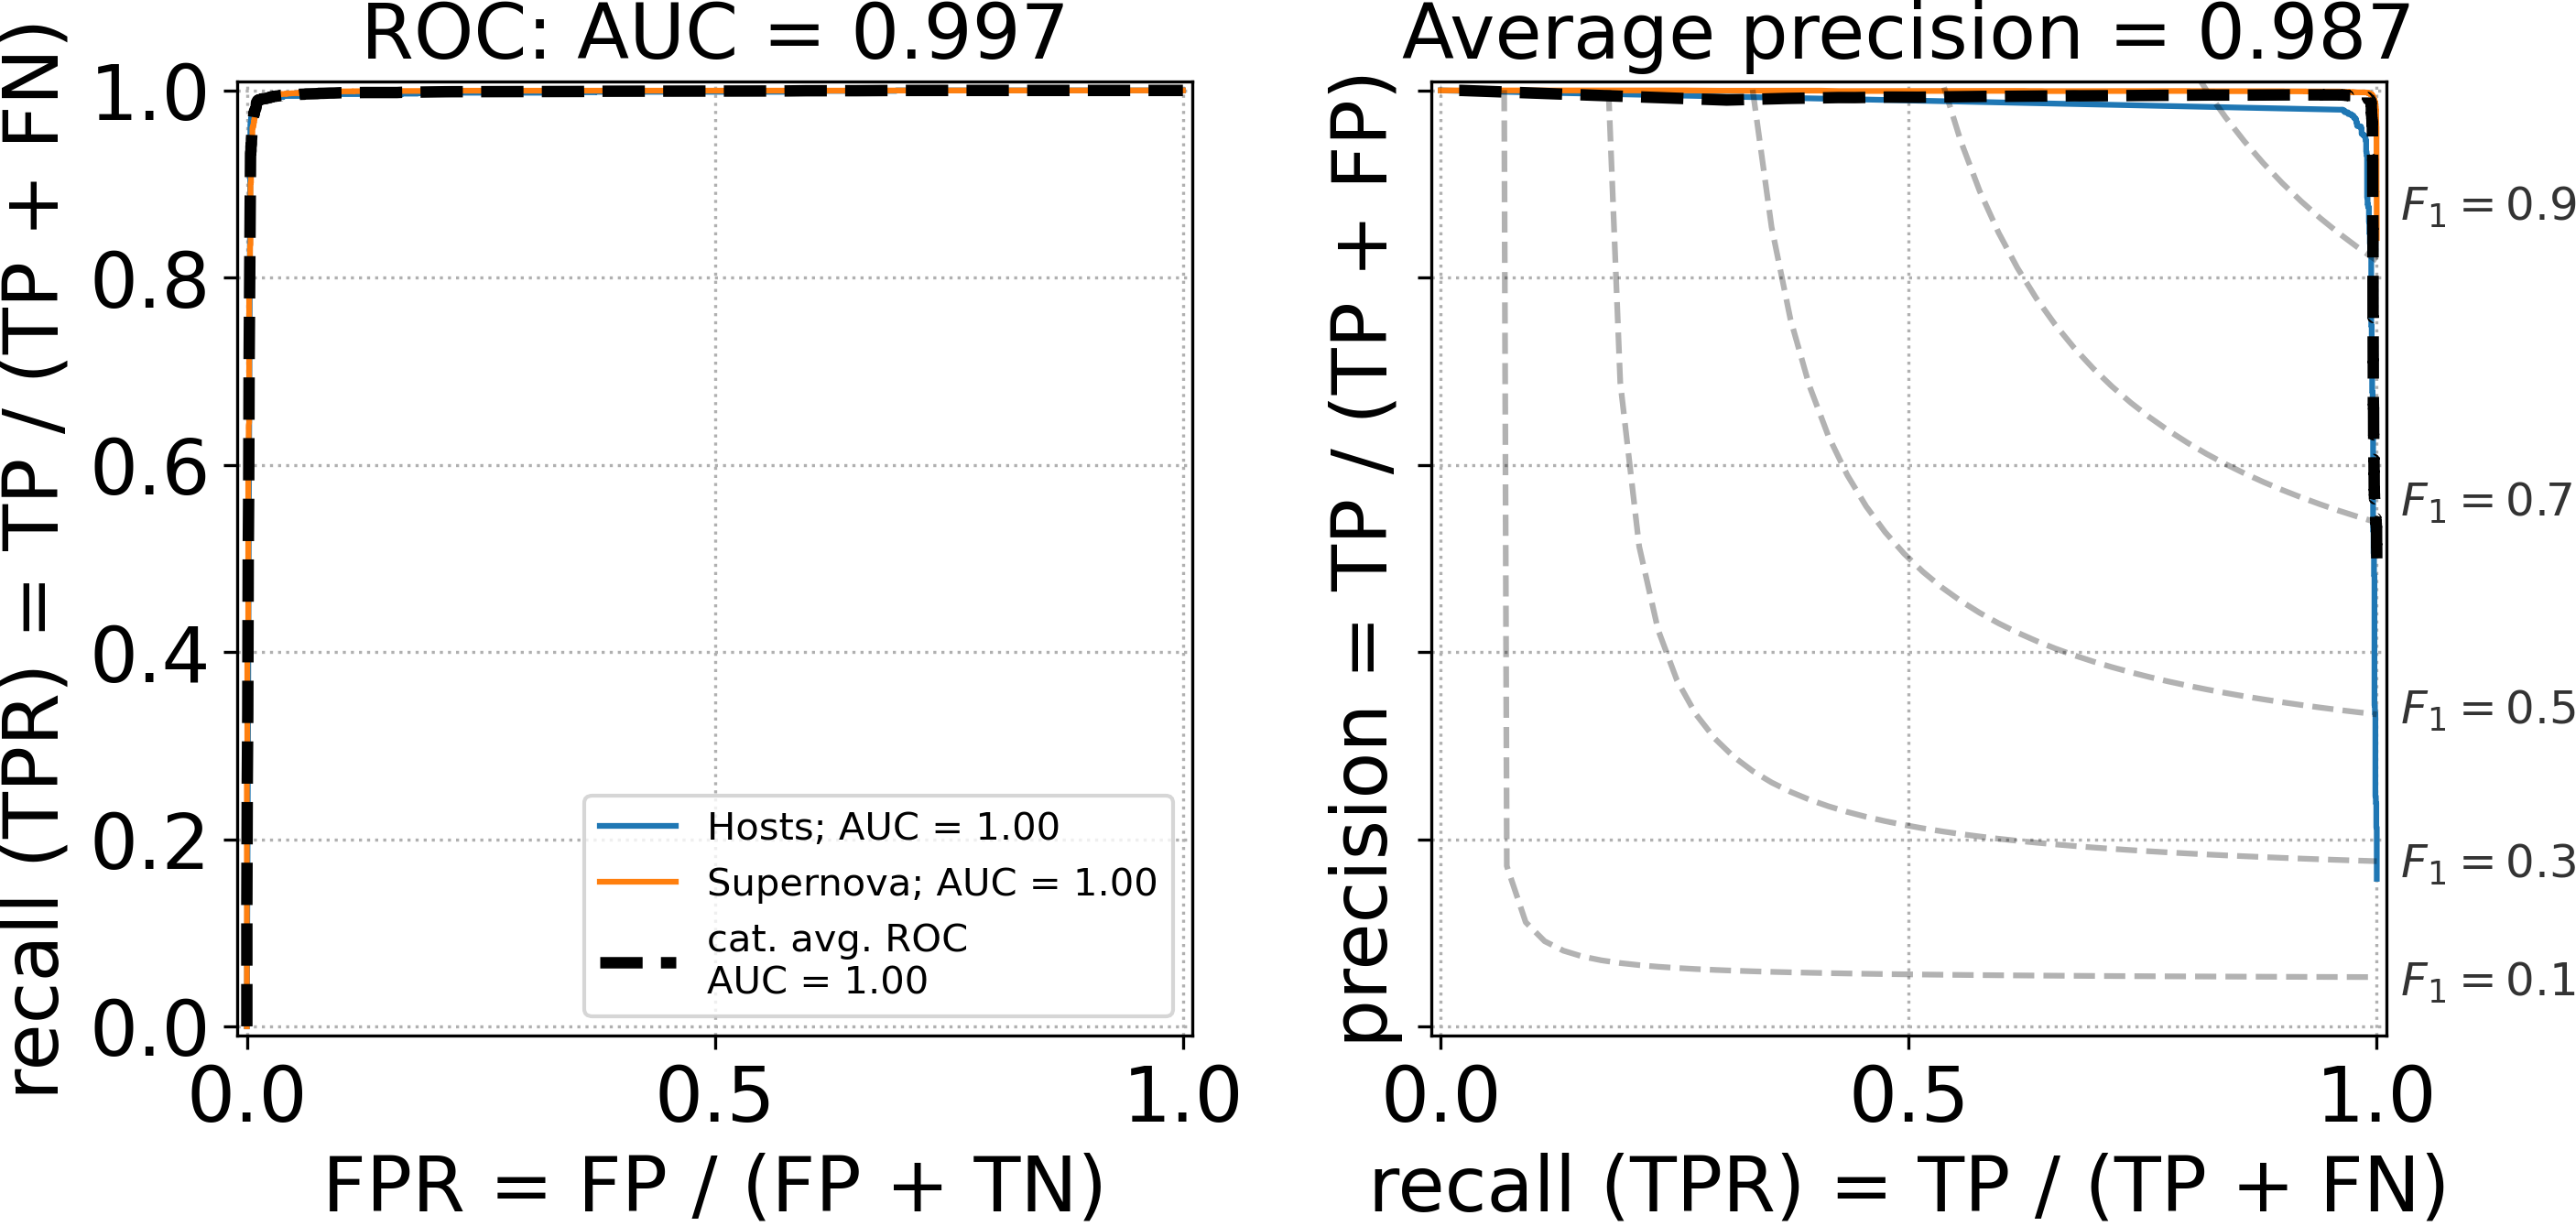
\includegraphics[height=2.7cm]{figures/v2_real/vit_model_V2rocfull_binary_e26.png}
        \quad
        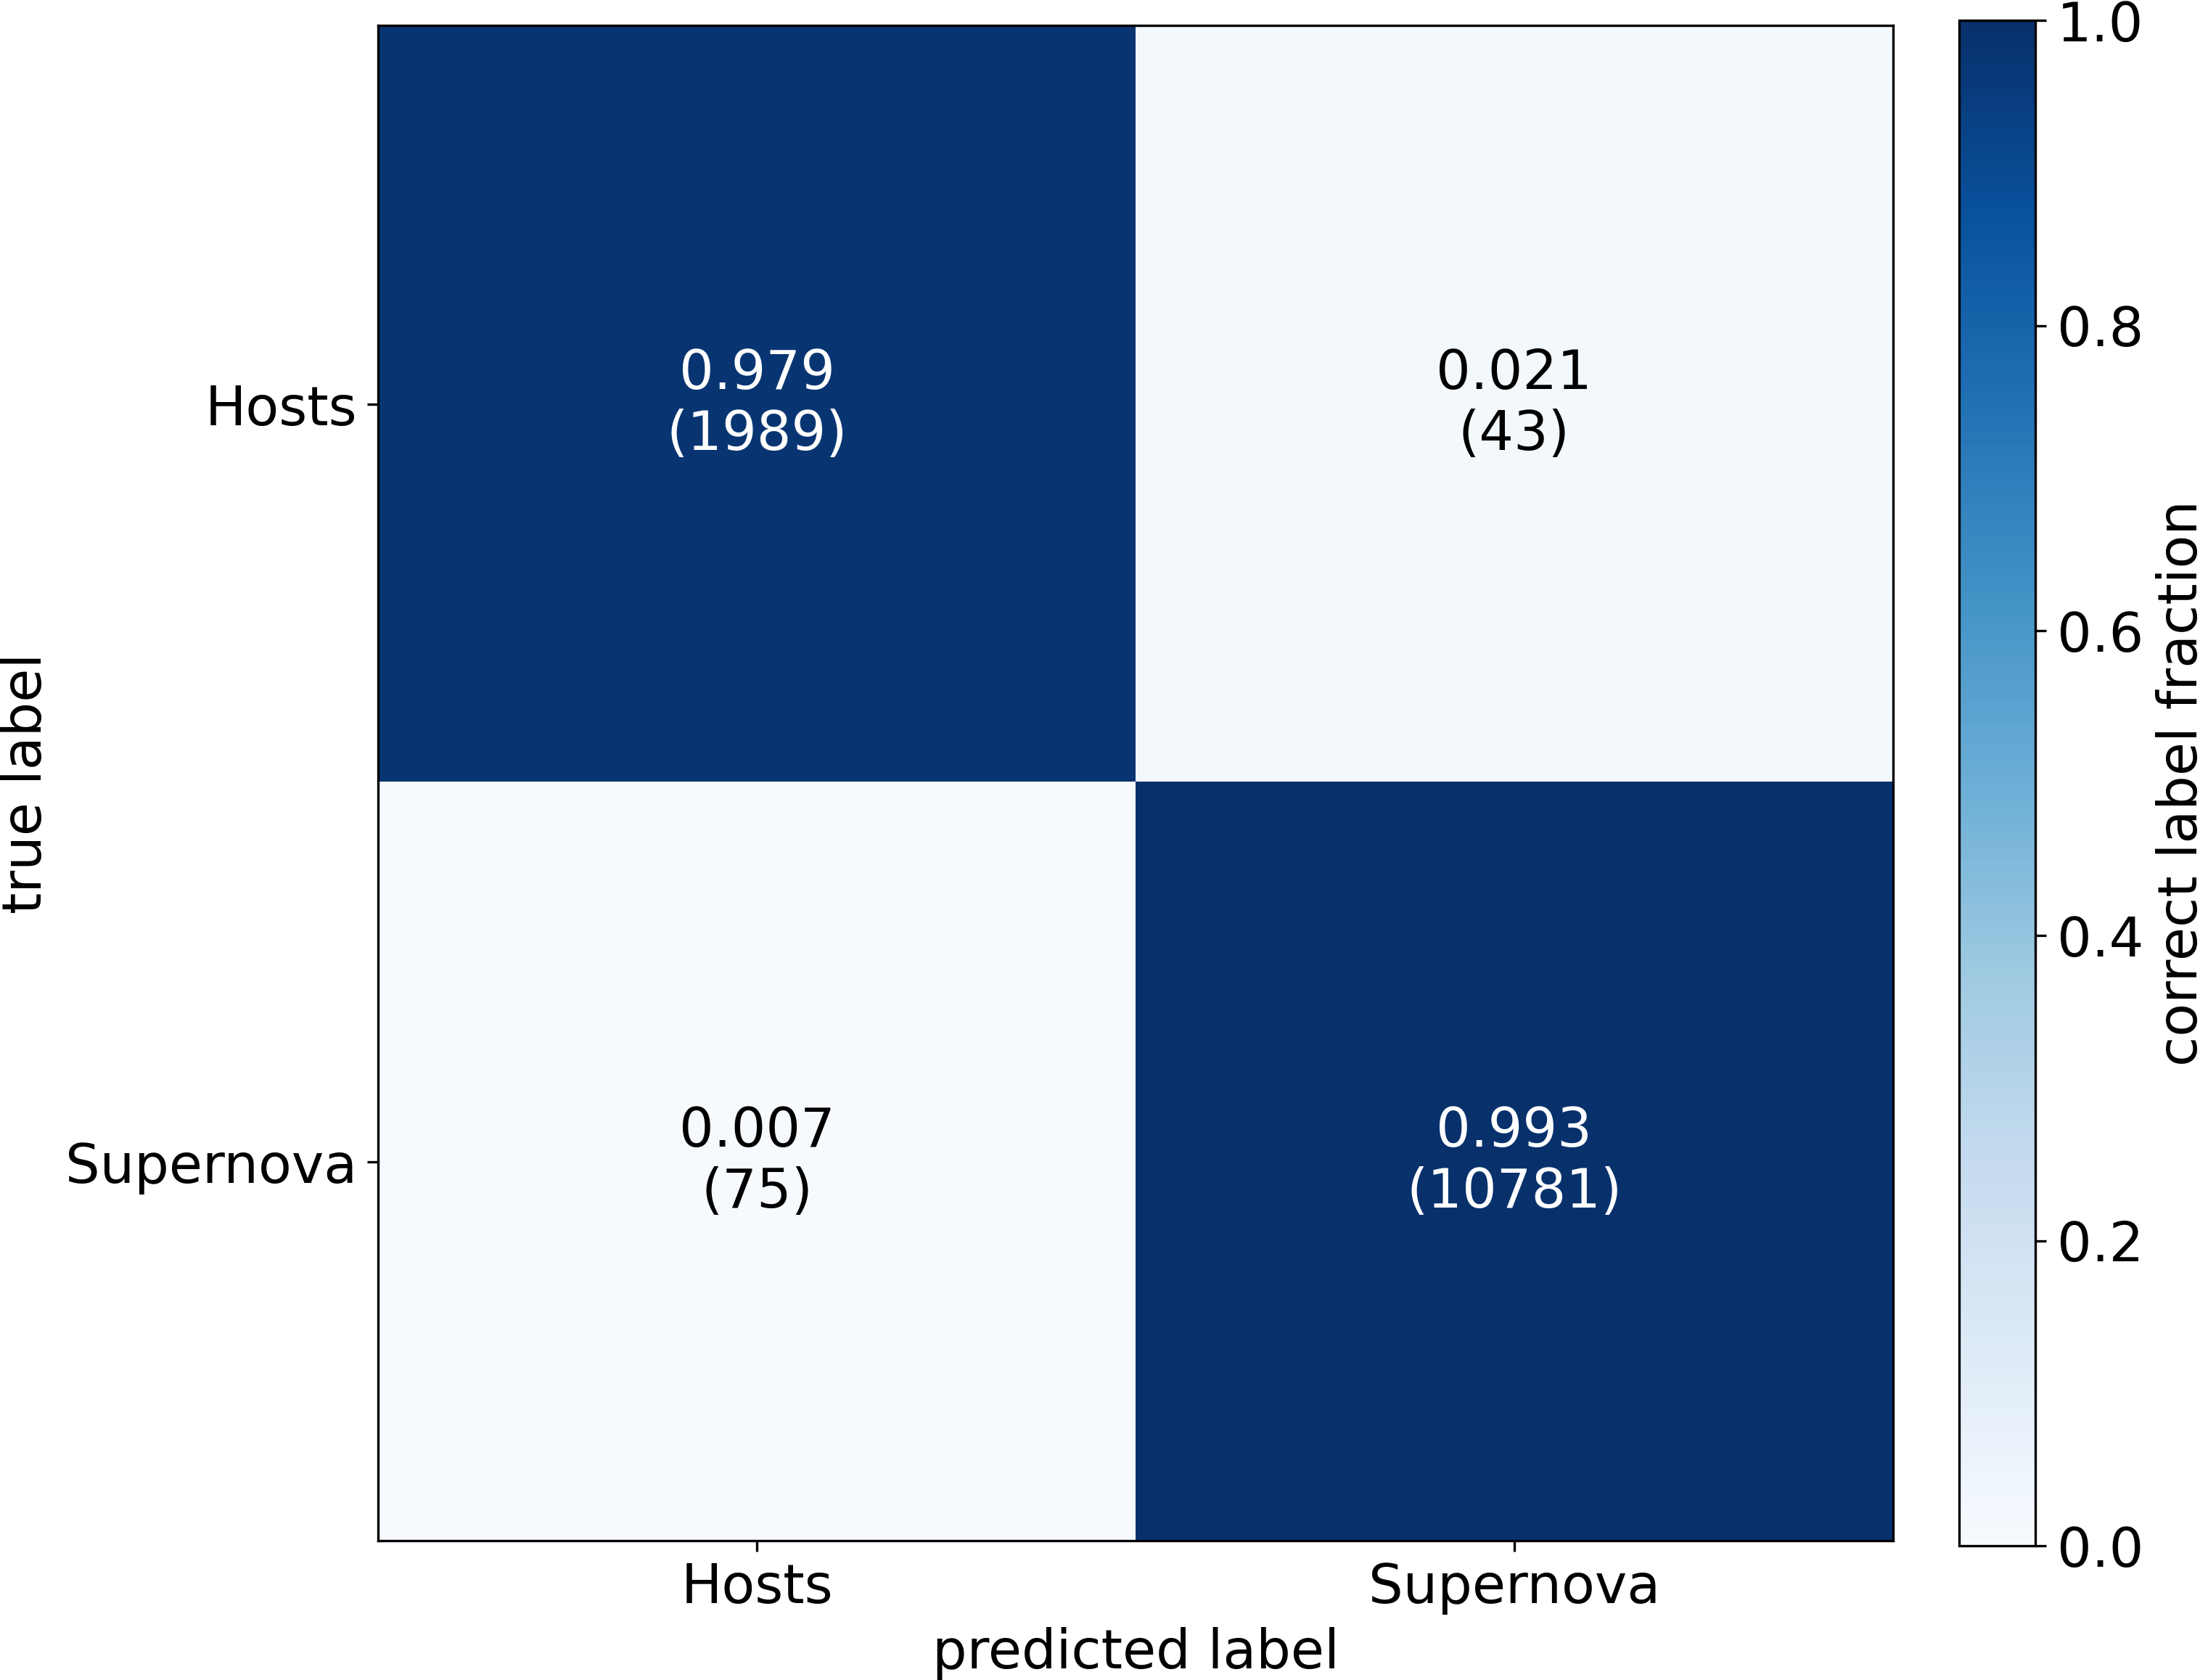
\includegraphics[height=2.7cm]{figures/v2_real/vit_model_V2cmfull_binary_e26.png}
        \caption{Spectral ViT V2 Binary Classifier\label{fig:v2_binary_qual}}
    \end{figure}
\end{frame}

\begin{frame}{Other Classifiers}
    \begin{figure}
        \centering
        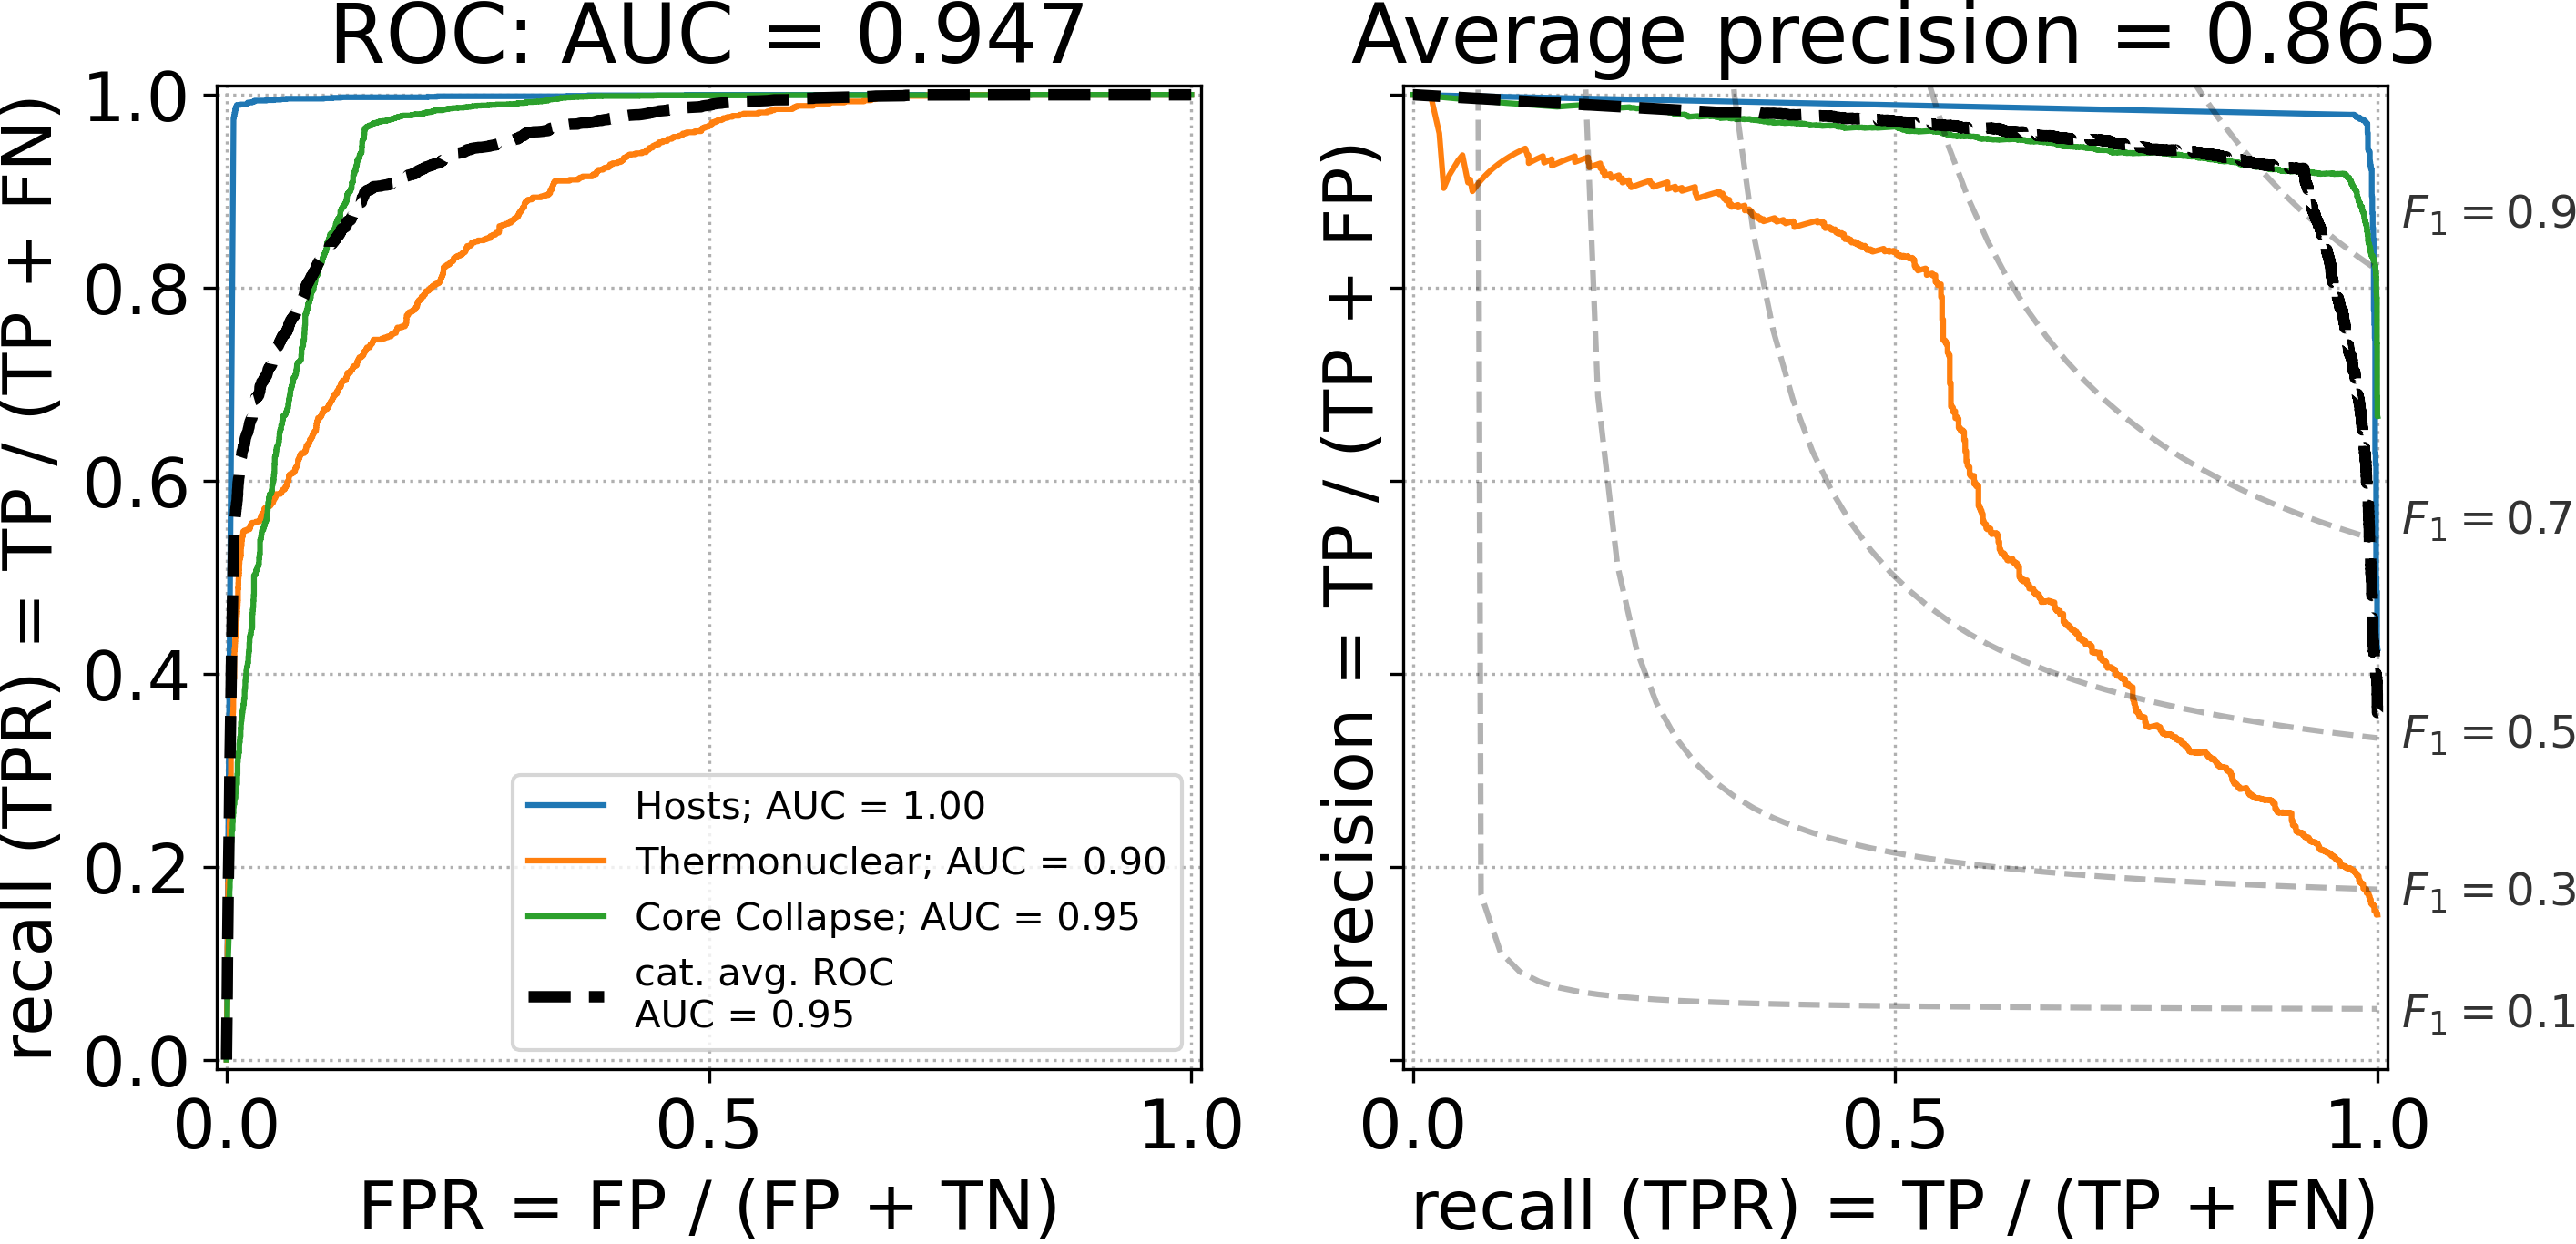
\includegraphics[height=2.5cm]{figures/v2_applications/vit_model_V2roc99_proj_e26.png}
        \quad
        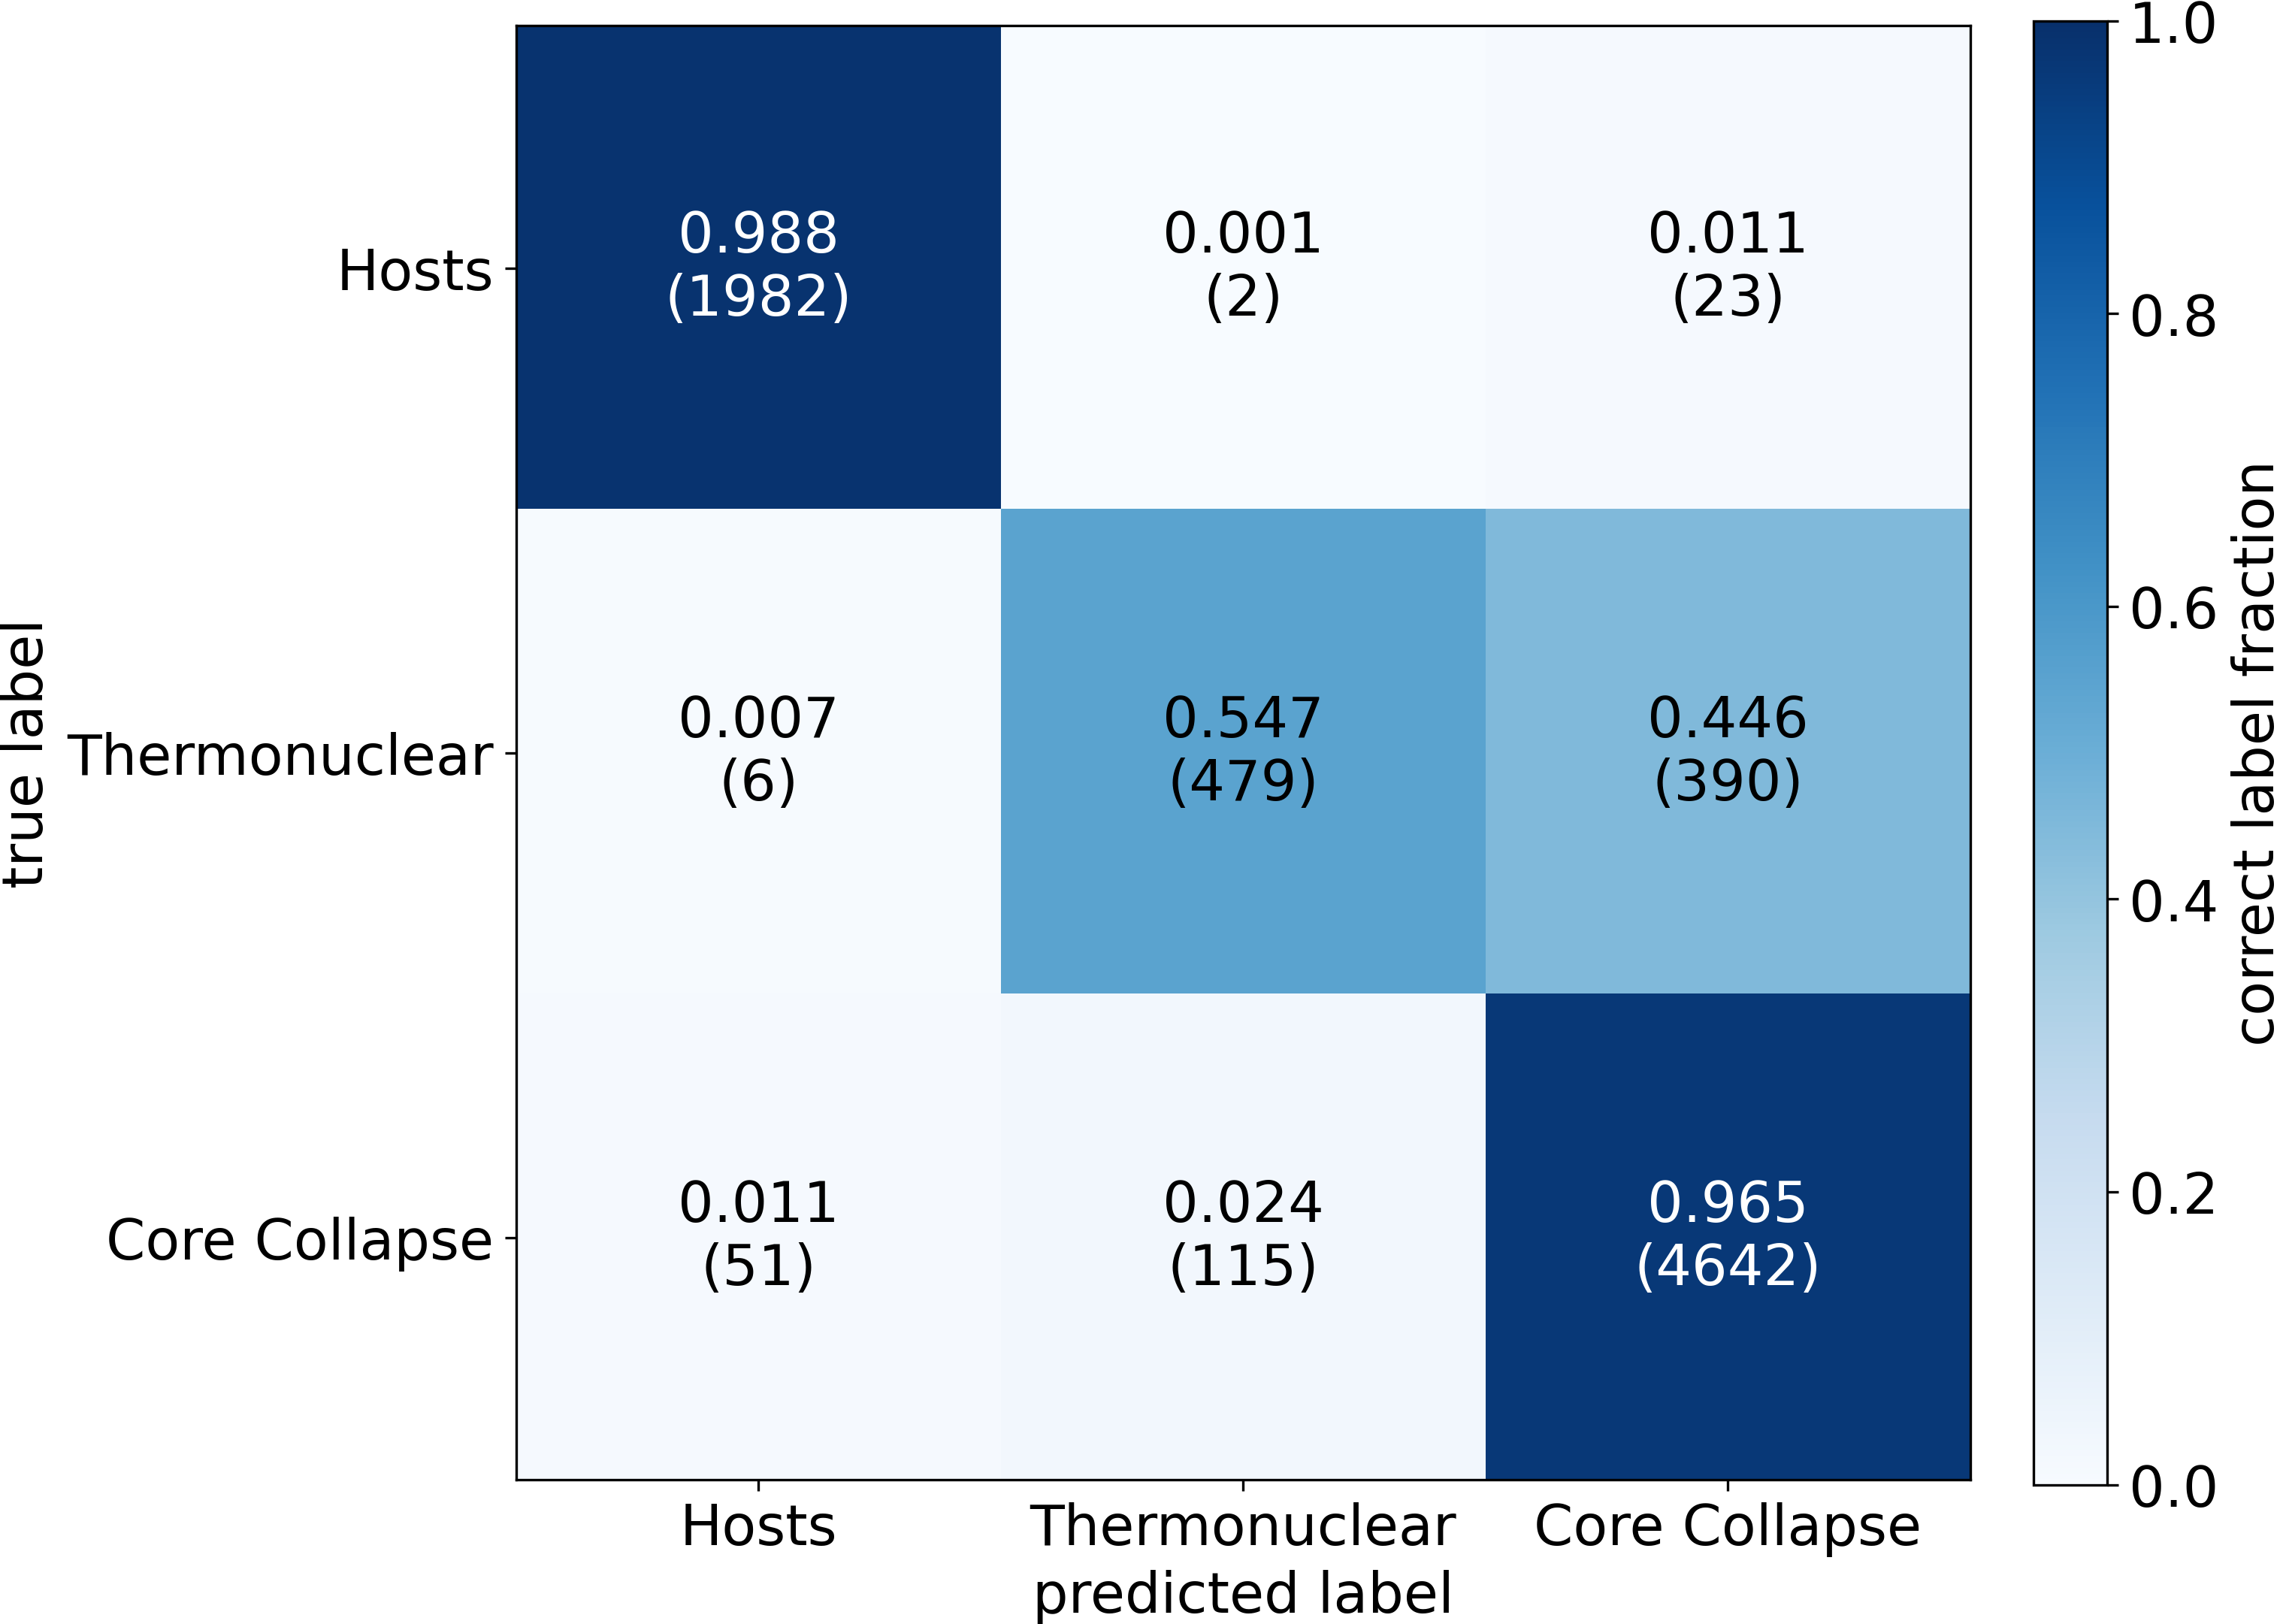
\includegraphics[height=2.5cm]{figures/v2_applications/vit_model_V2cm99_proj_e26.png}
        \caption{Spectral ViT V2 Progenitor Classifier (99\% confidence cut)\label{fig:v2_99_proj_qual}}
    % \end{figure}
    % \begin{figure}[t!]
    %     \centering
        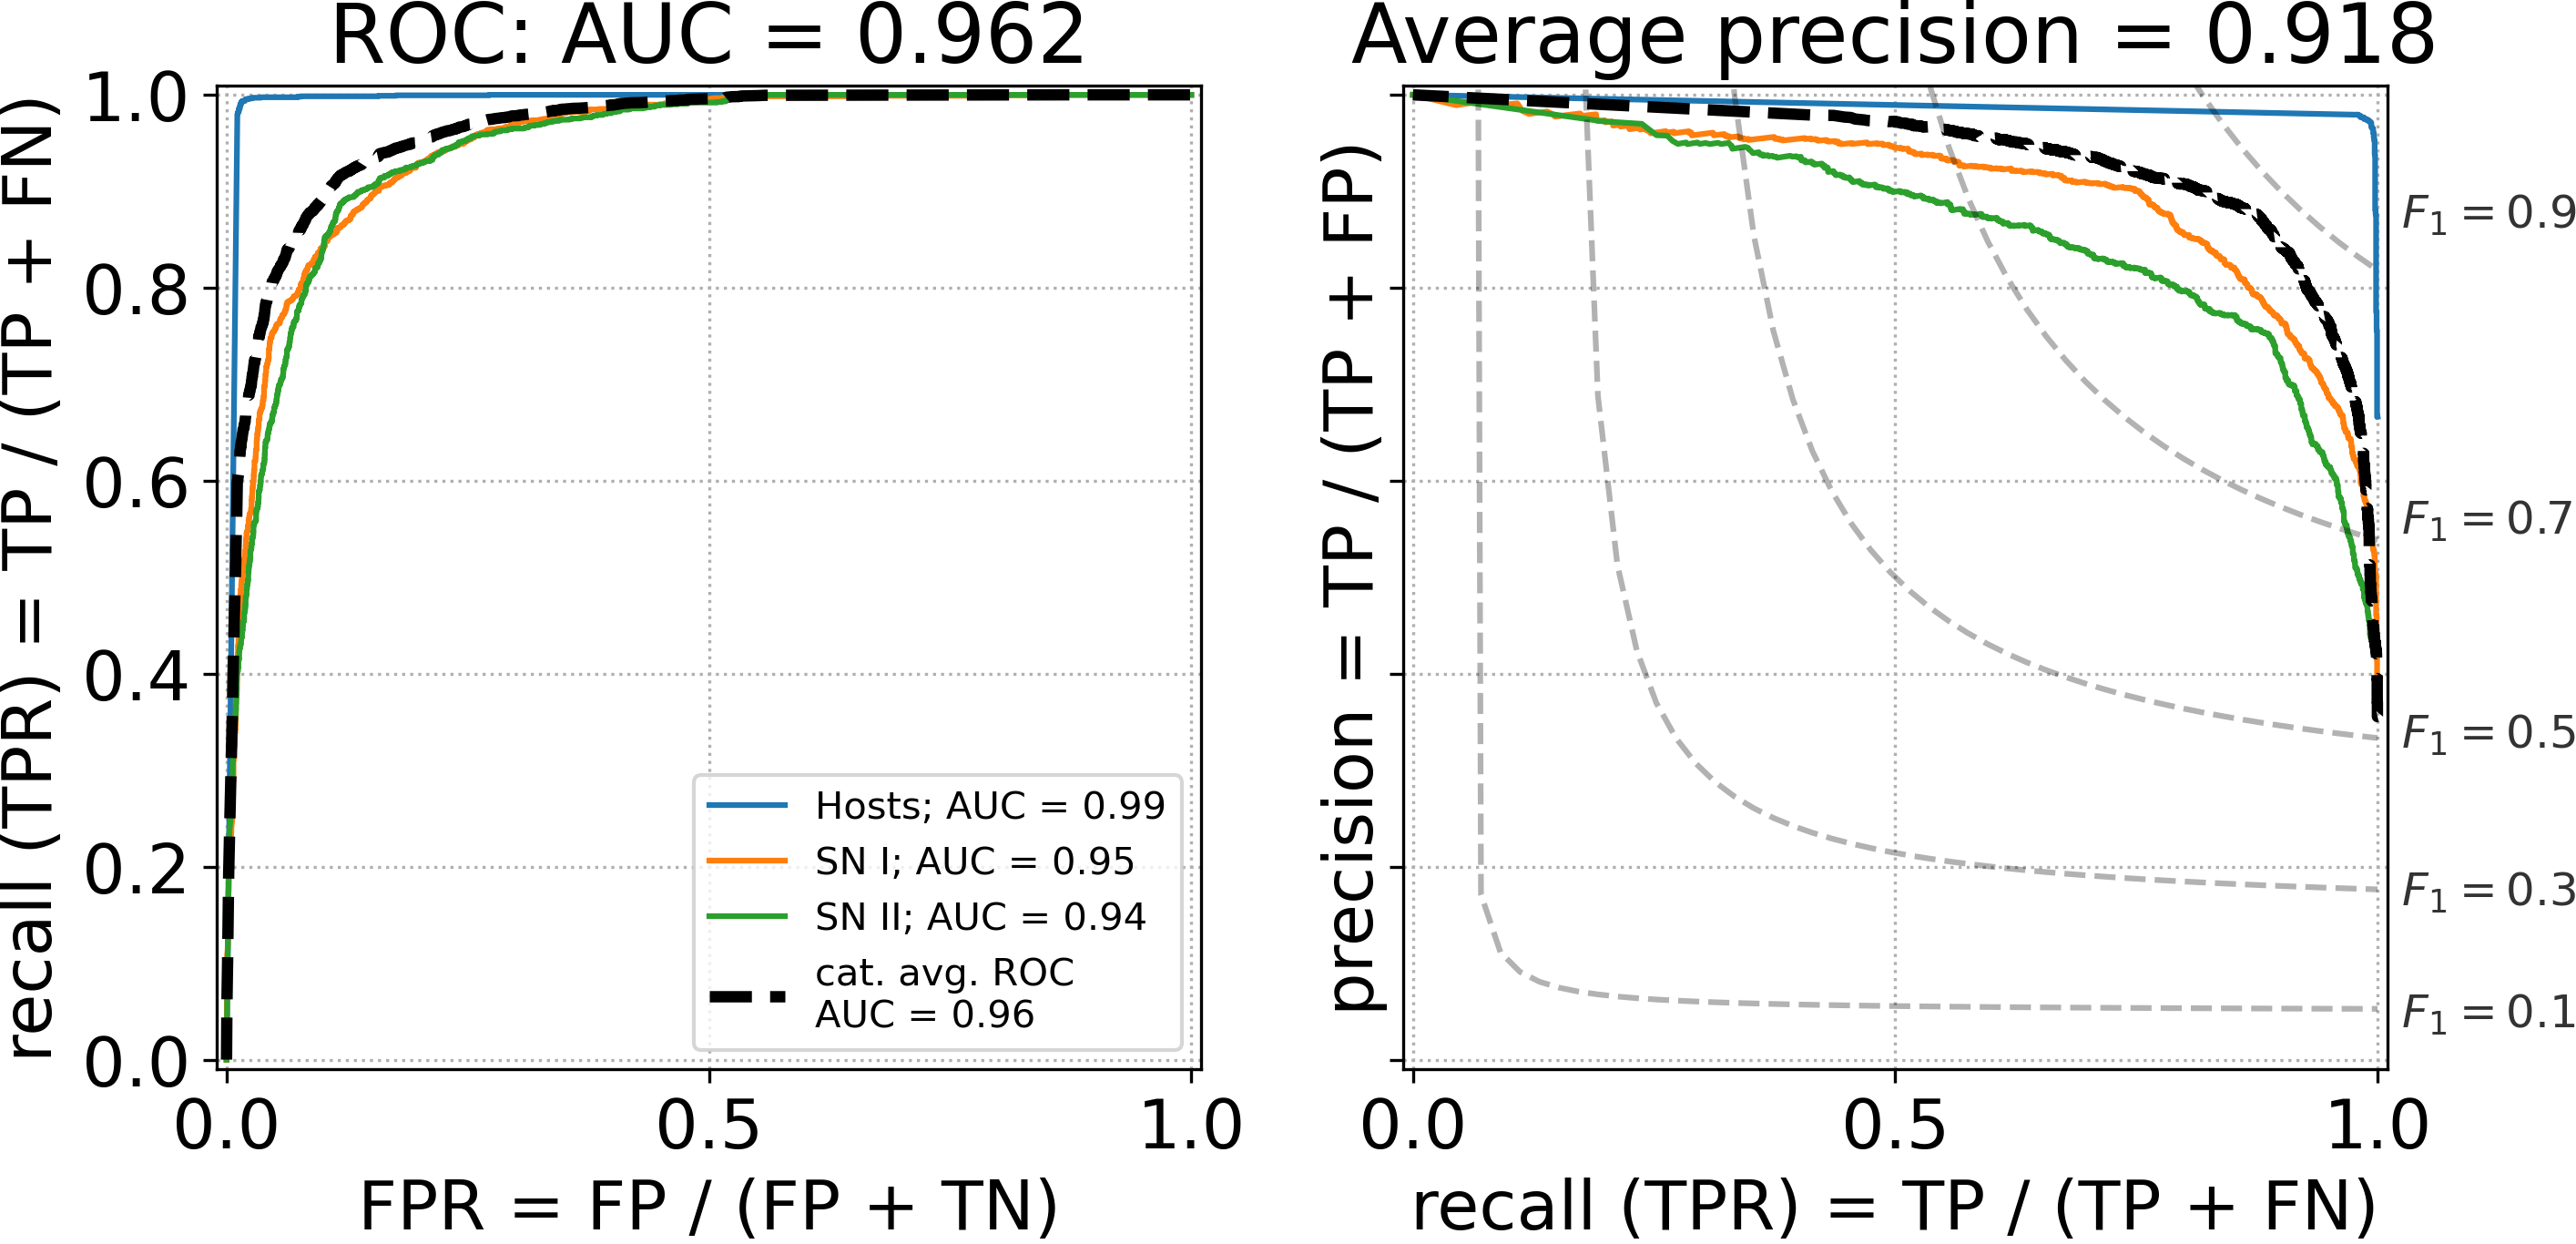
\includegraphics[height=2.5cm]{figures/v2_applications/vit_model_V2roc99_type_e26.png}
        \quad
        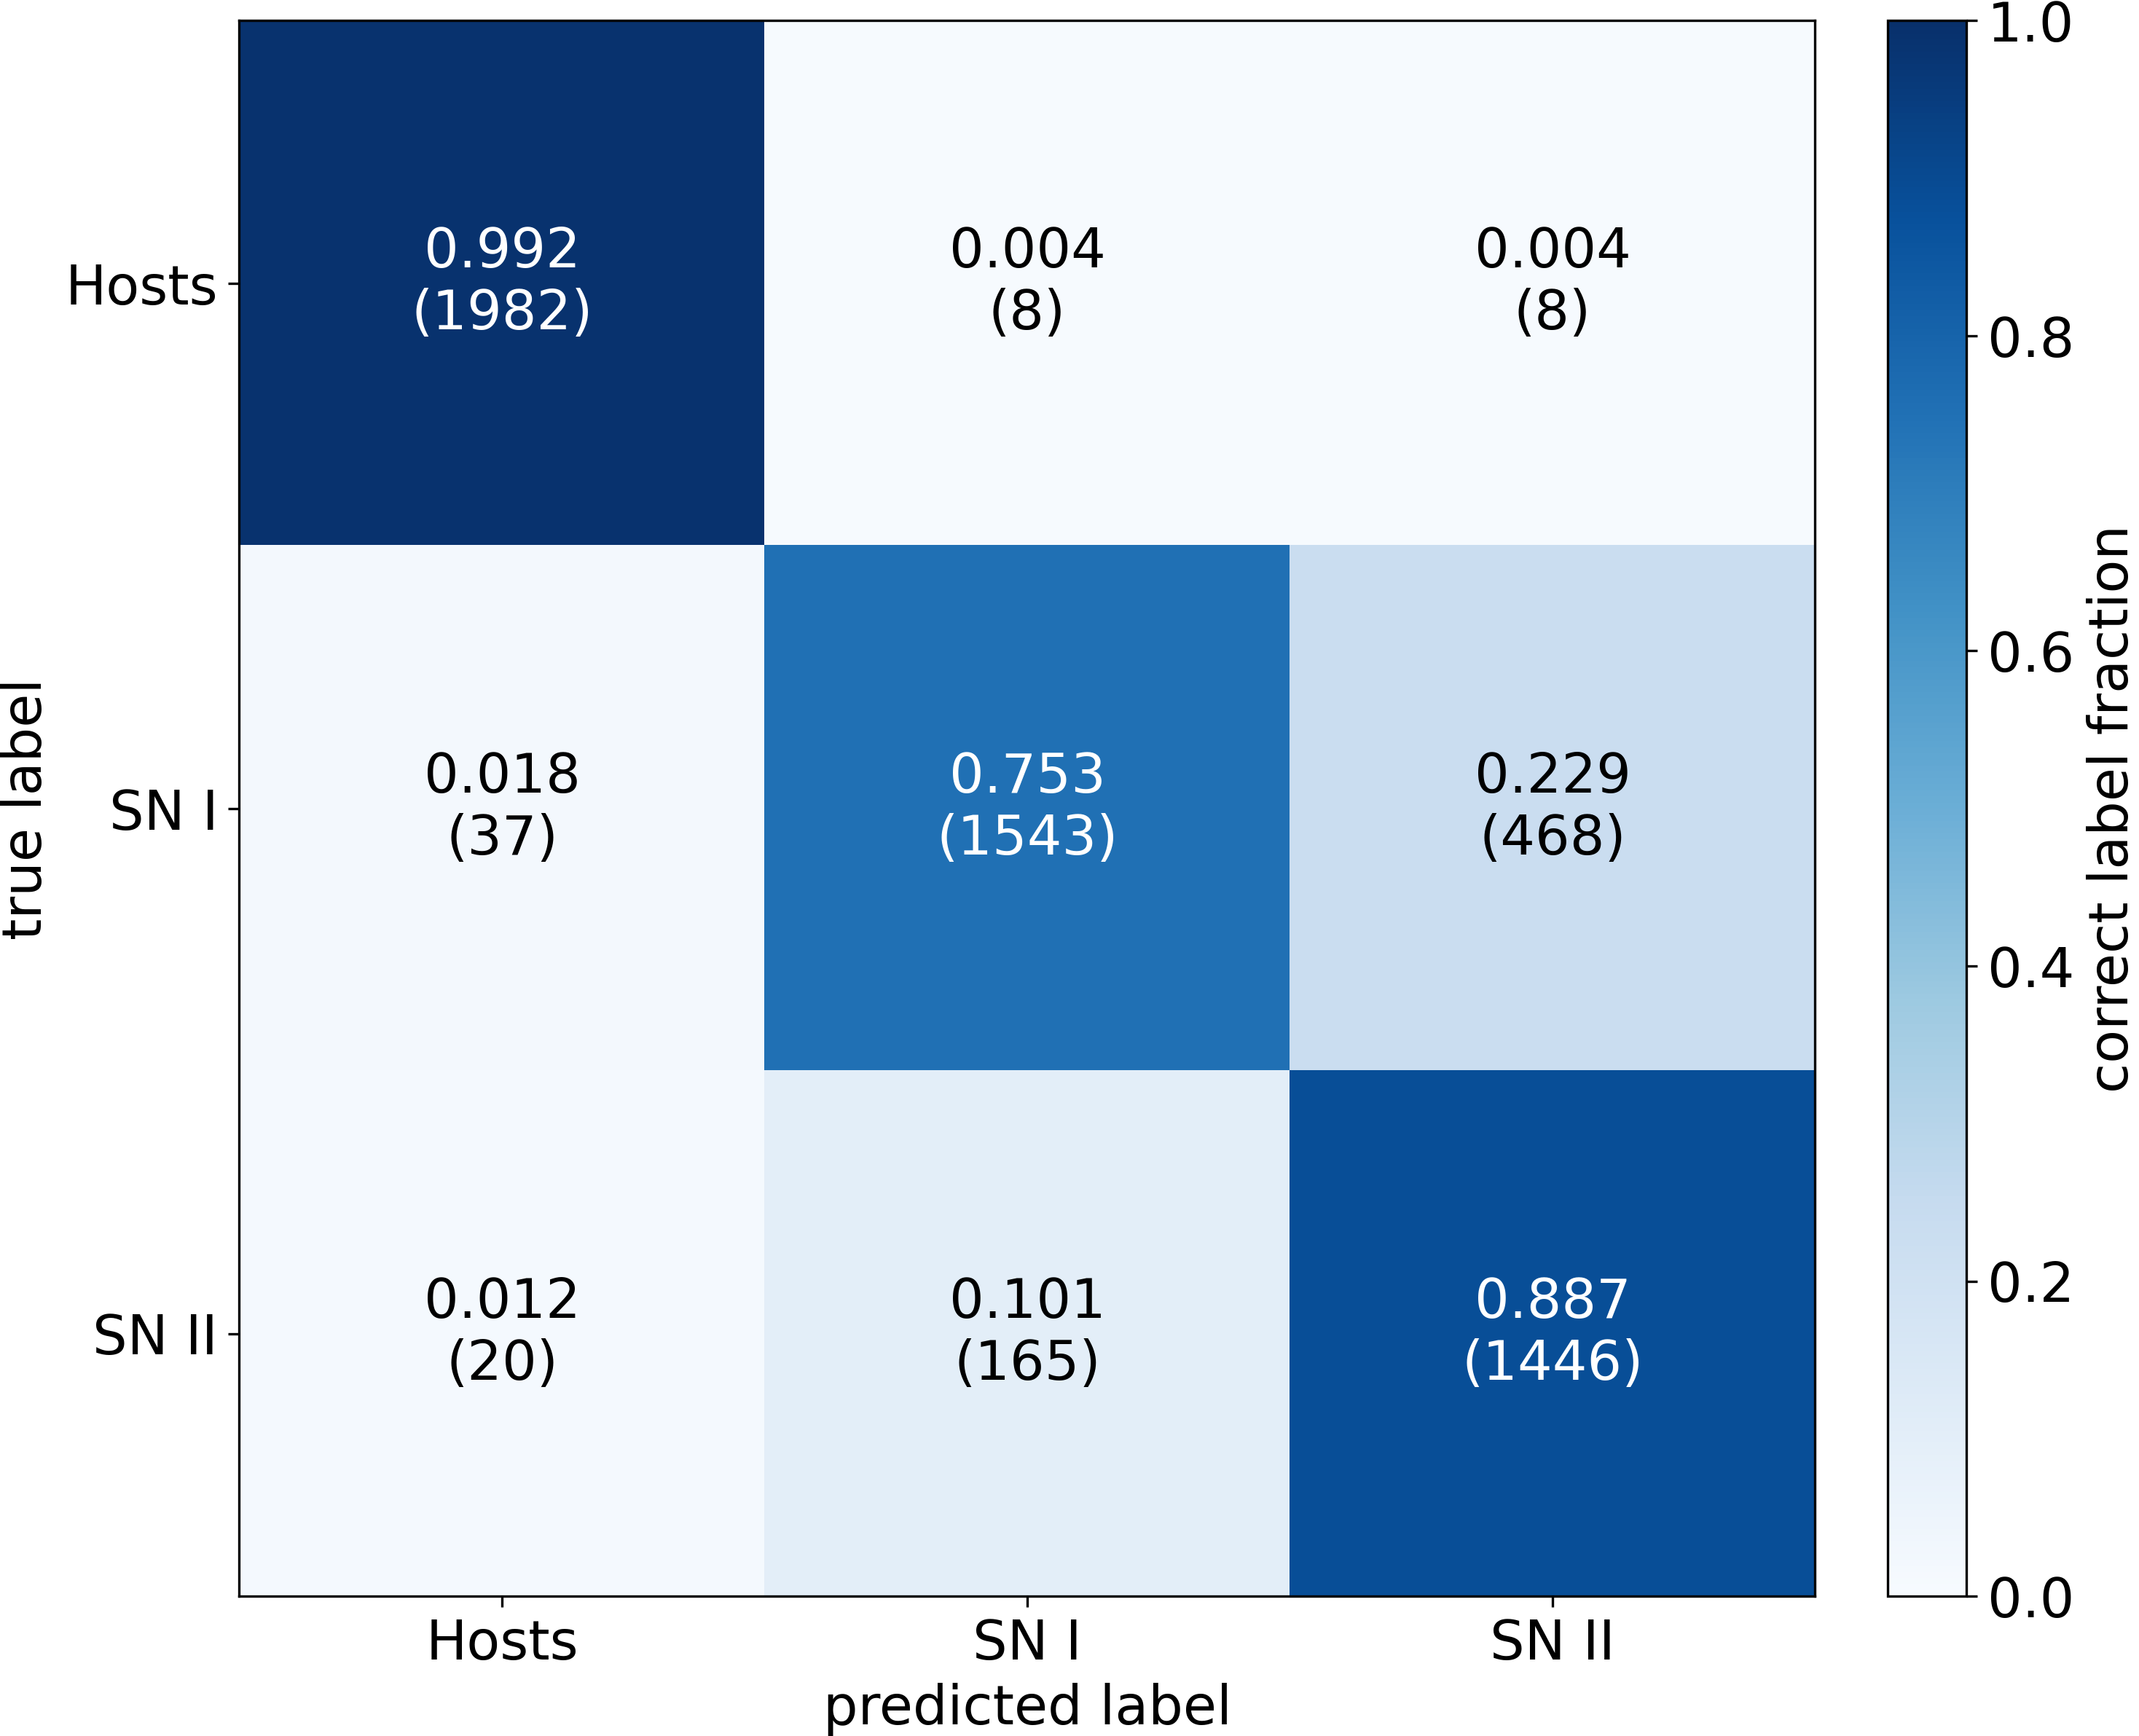
\includegraphics[height=2.5cm]{figures/v2_applications/vit_model_V2cm99_type_e26.png}
        \caption{Spectral ViT V2 Type Classifier (99\% confidence cut)\label{fig:v2_99_type_qual}}
    \end{figure}
\end{frame}



% \begin{figure}[h]
%     \centering
%     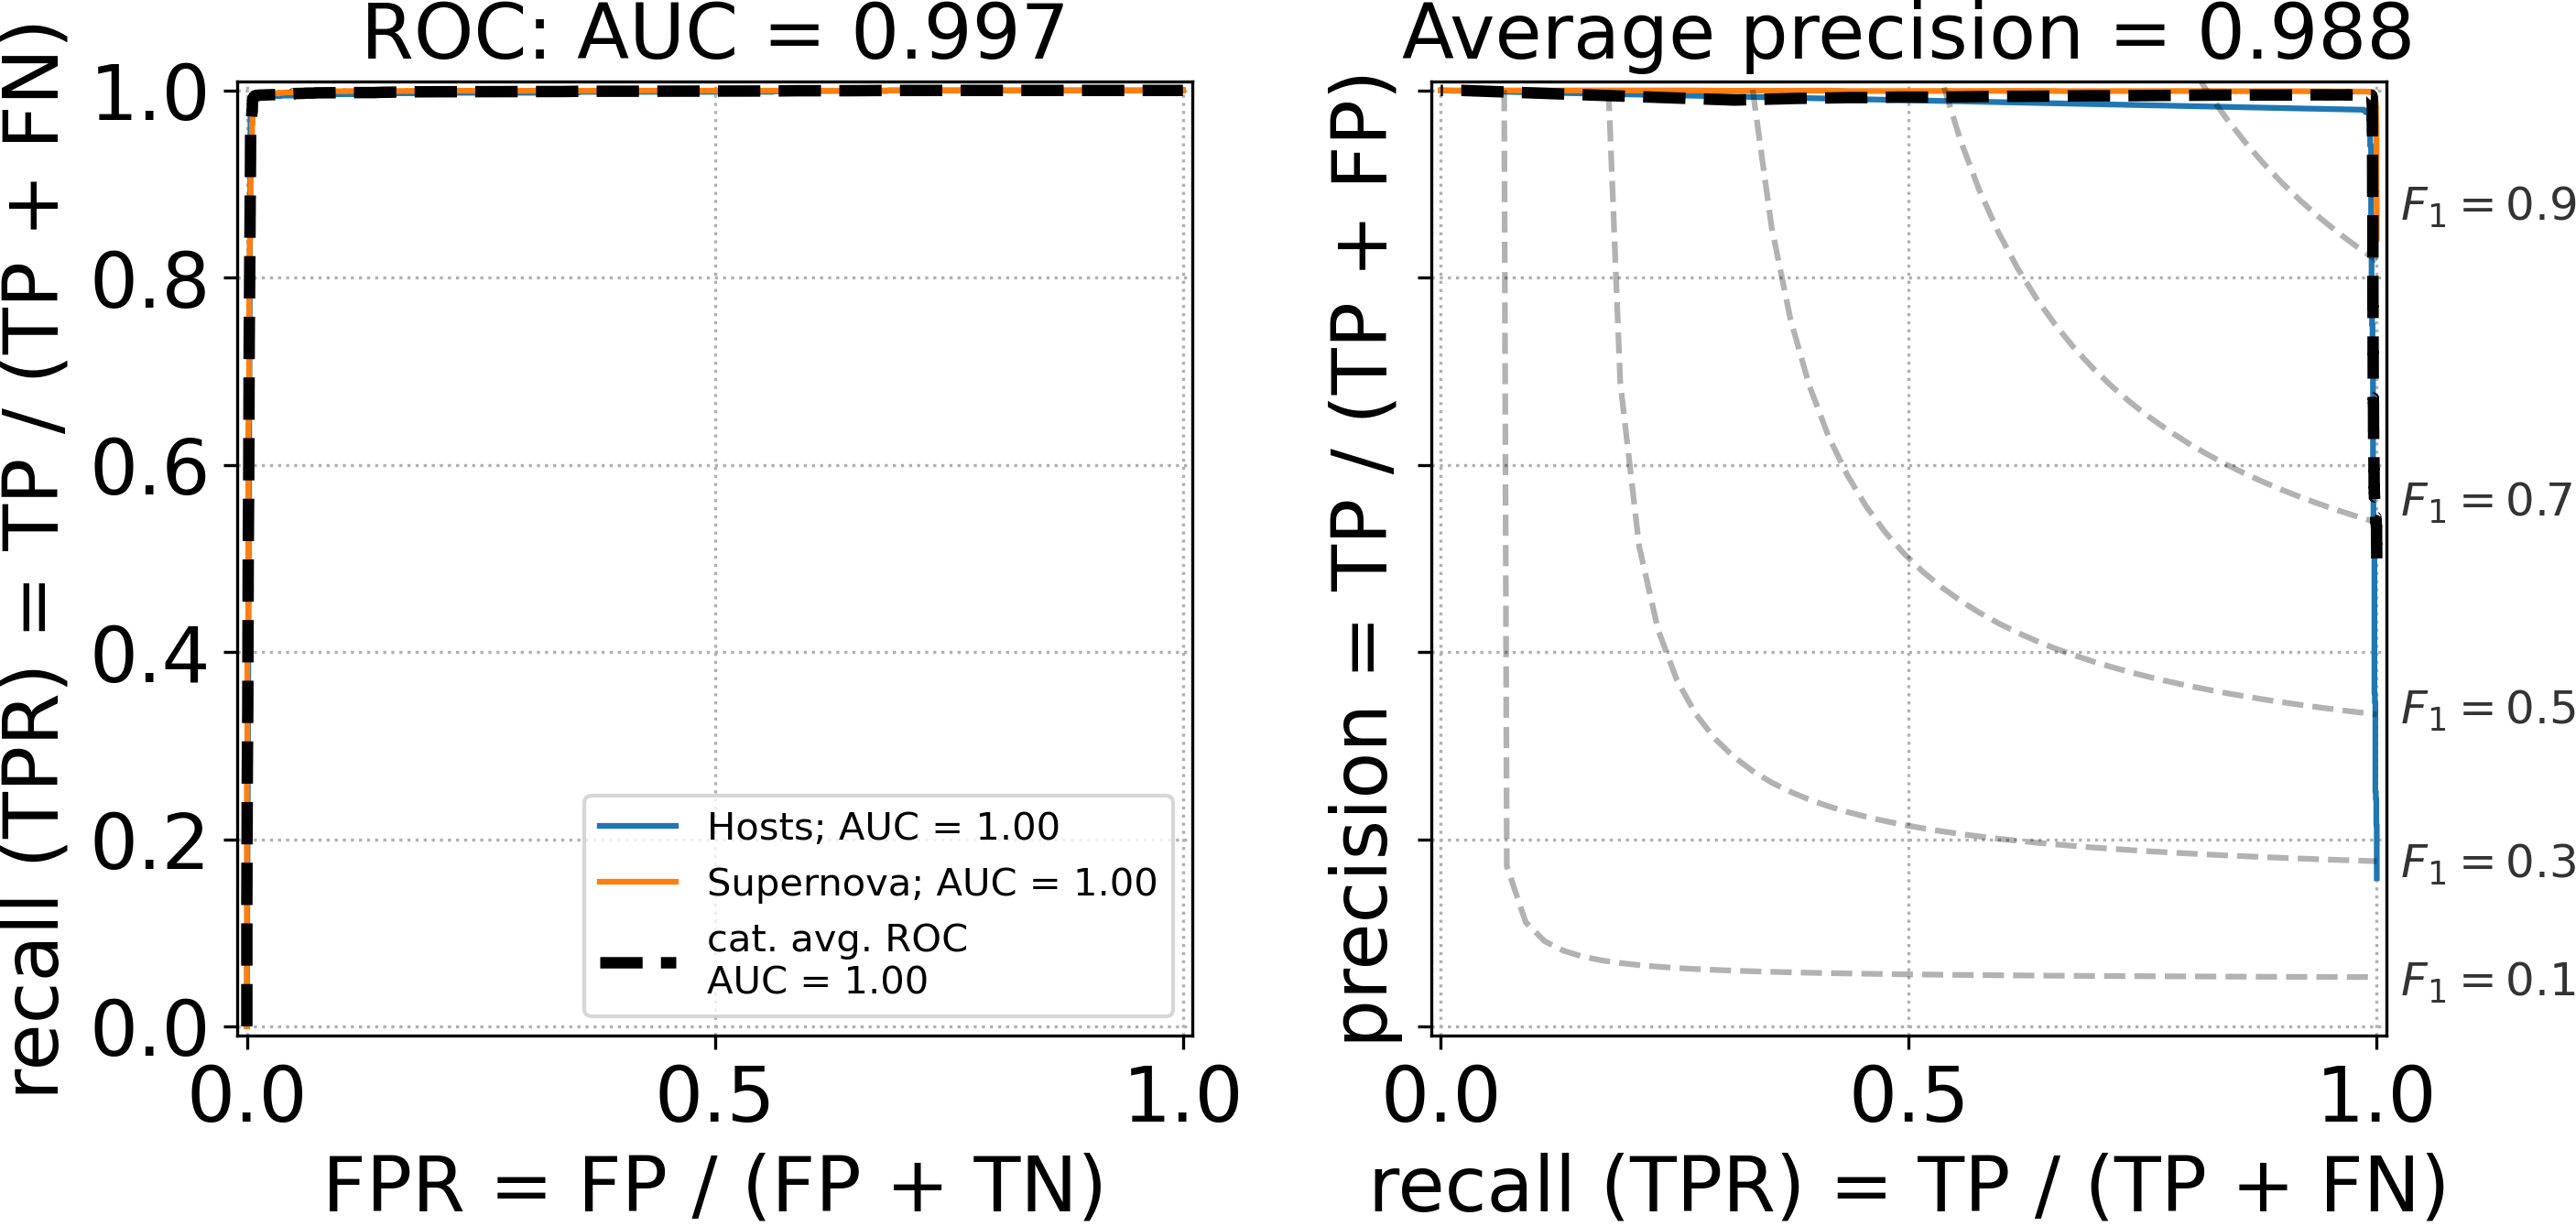
\includegraphics[height=2.7cm]{figures/v2_real/vit_model_V2roc9999_binary_e26.png}
%     \quad
%     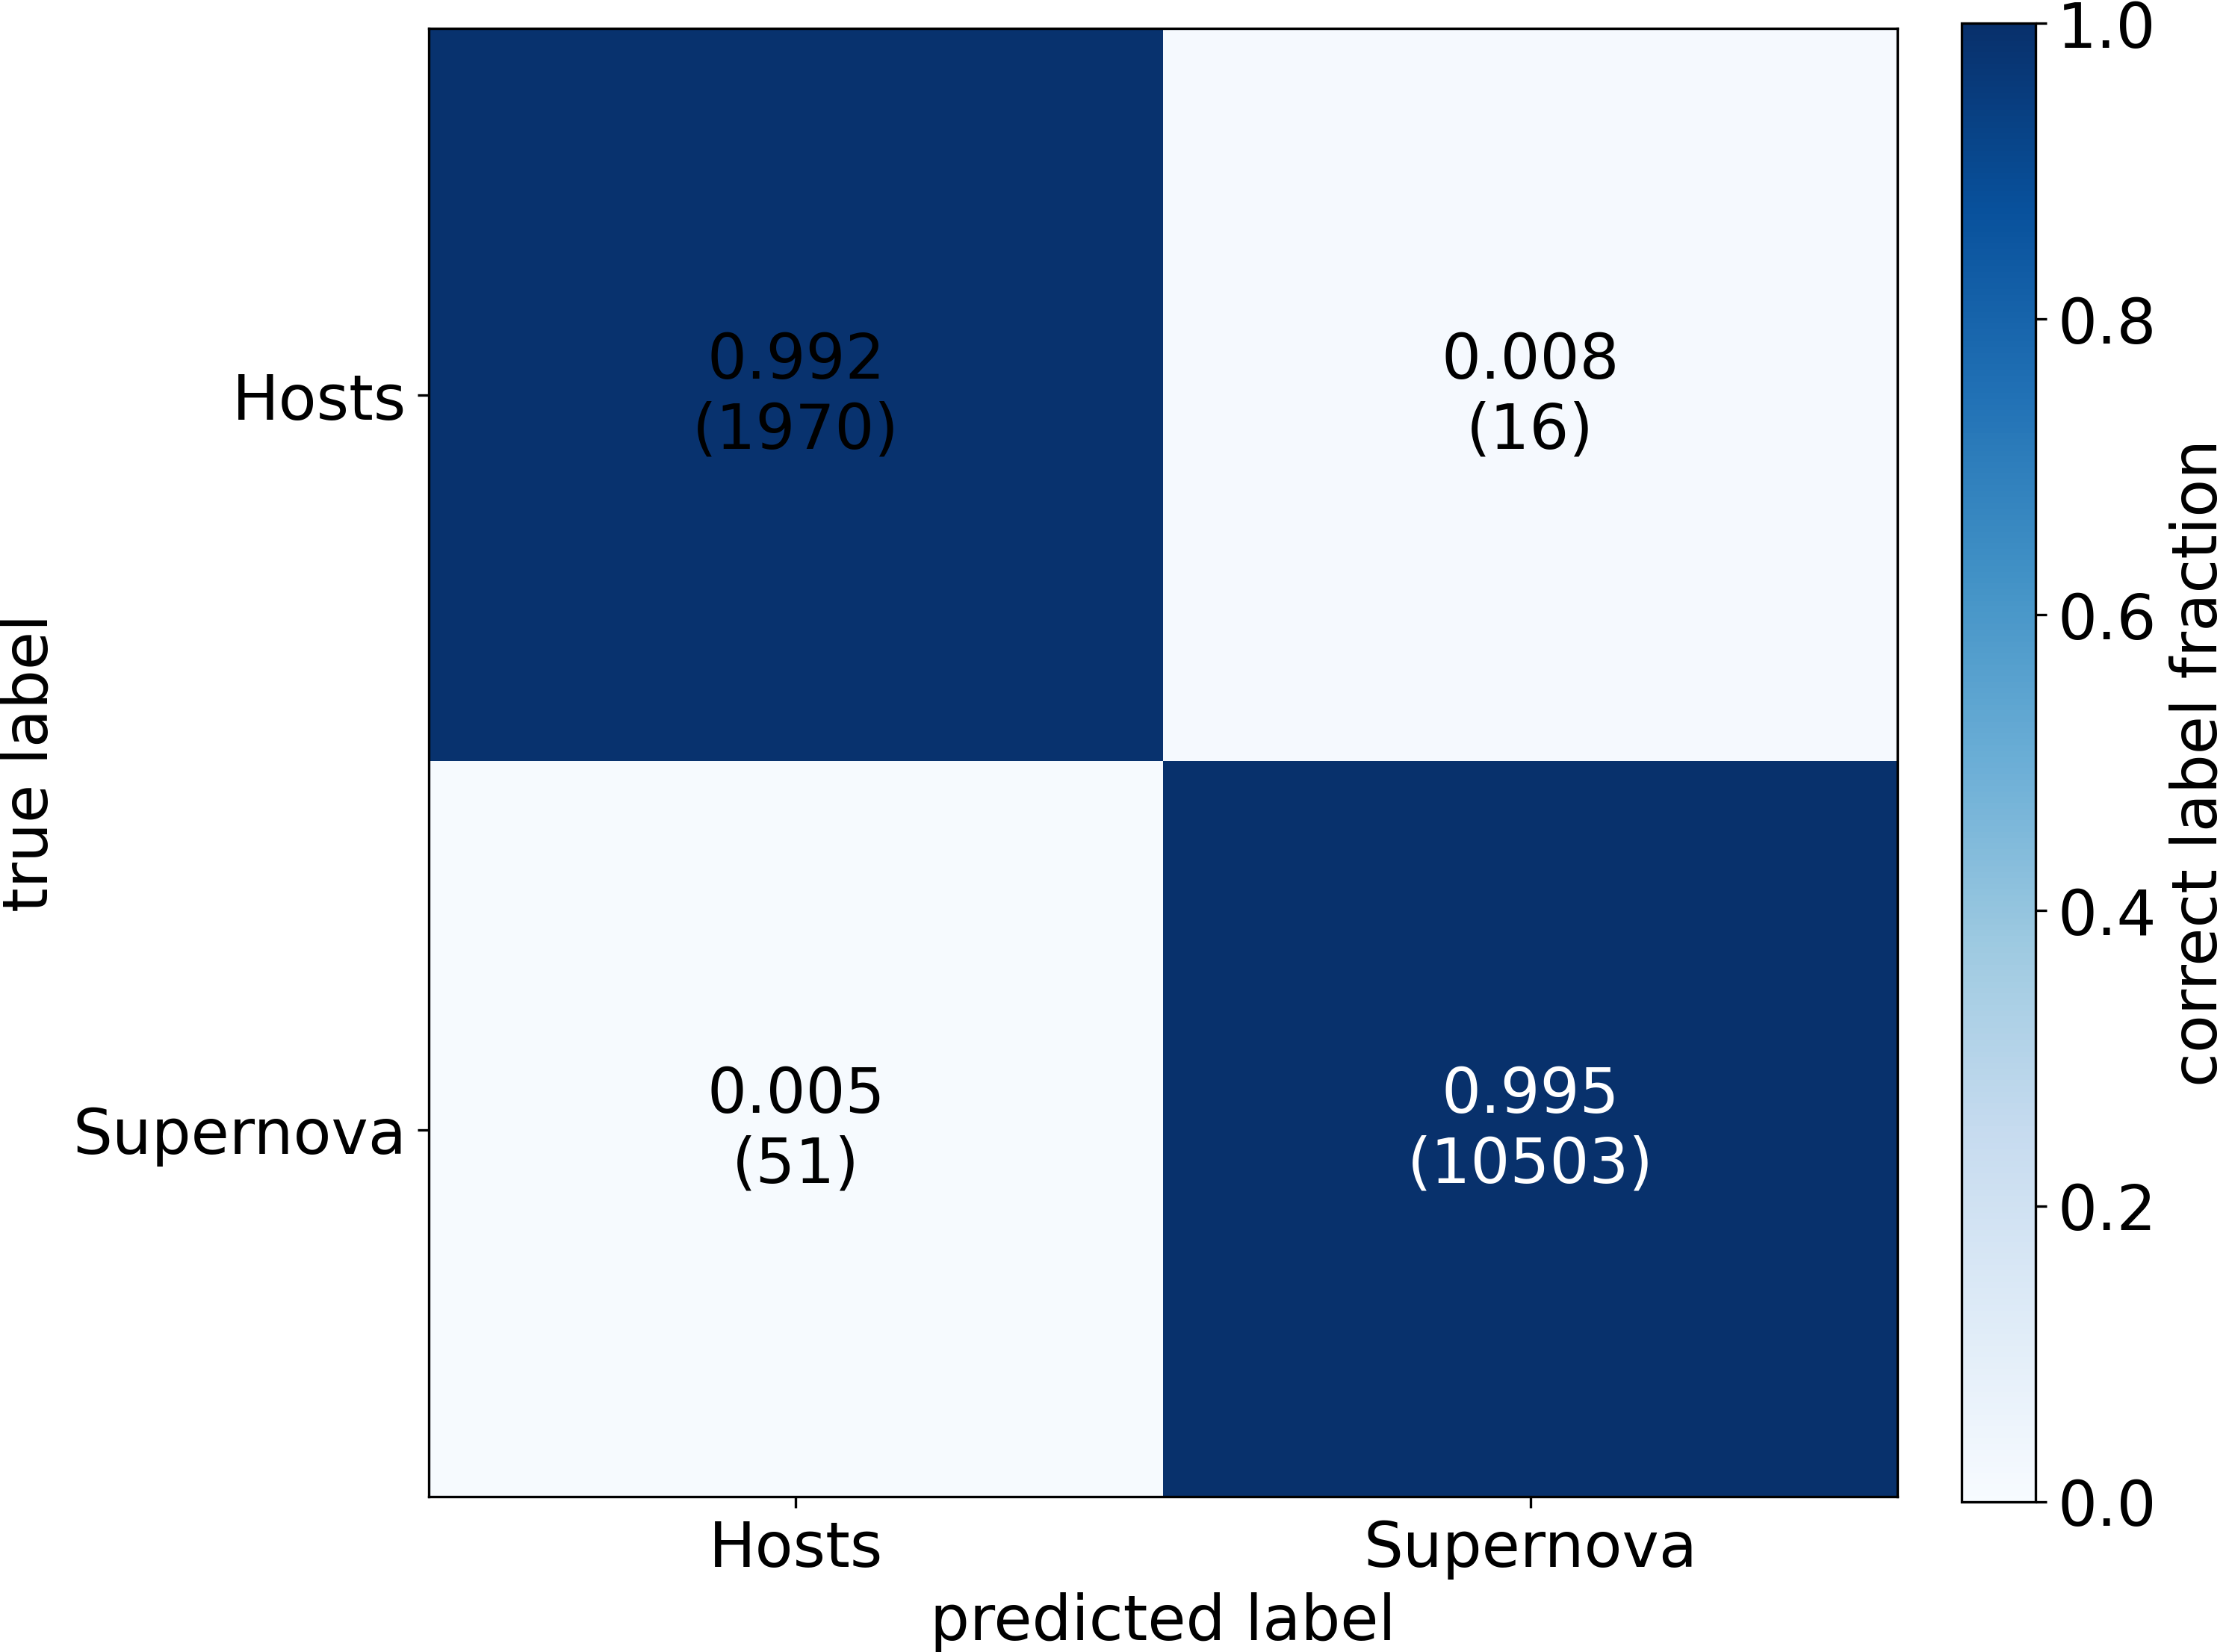
\includegraphics[height=2.7cm]{figures/v2_real/vit_model_V2cm9999_binary_e26.png}
%     \caption{Spectral ViT V2 Binary Diagnostics: ROC Curve (left) and Confusion Matrix (right) with a 99.99\% confidence
%     cut \label{fig:v2_binary_9999_qual}}
% \end{figure}


\begin{comment}
\begin{frame}
    \frametitle{Results}
    \small
    \begin{table}[]
        \centering
        \caption{Best performance after 25 epochs of training.}
        \resizebox{\linewidth}{!}{\begin{tabular}{lccc}
	\toprule
    \textbf{Spam} & \textbf{Ni} & \textbf{Swallow} & \textbf{Shrubbery} \\
    \midrule
    A & 1 & 2 & 3 \\
    \midrule
    E & 3 & 4 & 5 \\
    C & 6 & 9 & 3 \\
    \midrule
    M & 4 & 1 & 1 \\
    \bottomrule
\end{tabular}}
    \end{table}
\end{frame}
%%%%%%%%%%%%%%%%%%%%%%%%%%%%%%%%%%%%%%%%%%%%%%%%%%%%%%%%%%%%%%%%%%%%%%%%
\begin{frame}
    \frametitle{Results -- Classification}
    \begin{figure}[t]
        \centering
        
\includegraphics[width=0.8\linewidth]{figures/blackbox.jpeg}
        \caption{Predictions after training on the full HAM10000 dataset}\label{fig:preds}
    \end{figure}

    \begin{figure}[b]
        \centering
        
\includegraphics[width=0.8\linewidth]{figures/blackbox.jpeg}
        \caption{Predictions after training on a shrunken HAM100000 dataset}\label{fig:predsSmall}
    \end{figure}
\end{frame}
%%%%%%%%%%%%%%%%%%%%%%%%%%%%%%%%%%%%%%%%%%%%%%%%%%%%%%%%%%%%%%%%%%%%%%%%
\begin{frame}
    \frametitle{Results -- Segmentation}
    \begin{figure}[h]
        \centering
        
\includegraphics[width=.6\linewidth]{figures/blackbox.jpeg}
        \caption{Segmentation Results with Dice scores (Equation\ref{eqn:DiceScore})}\label{fig:seg}
    \end{figure}
\end{frame}
\end{comment}